%% $Id: hvfloat.tex 126 2021-06-29 12:56:04Z herbert $
\listfiles
\errorcontextlines=100
\documentclass[twoside,paper=a4,usegeometry]{scrartcl}
\usepackage{fontspec}
\usepackage{libertinus}
%\usepackage[scaled=0.85]{beramono}
\setmonofont[Scale=MatchLowercase,FakeStretch=0.9]{DejaVu Sans Mono}

\usepackage{microtype}
\usepackage[english]{babel}

\usepackage[marginparwidth=3cm,bottom=2cm,top=1cm,includeheadfoot]{geometry}


\usepackage[automark]{scrlayer-scrpage}
\pagestyle{scrheadings}

\usepackage{listings}
%
\lstset{%
    language=[LaTeX]TeX,%
    showstringspaces=false,%
    tabsize=5,%
    backgroundcolor=\color{black!15},
%    frame={tb},%
    lineskip=-1pt,%
    extendedchars=true,%
    basicstyle={\small\ttfamily},%
    numbers=left,%
    stepnumber=1,%
    numberstyle=\tiny,%
    xleftmargin=2em,%
    breaklines=true,
    }
%

\usepackage{graphicx}
\usepackage{placeins}
\usepackage{ragged2e}
\usepackage{xcolor}
\usepackage{url}
\usepackage{booktabs,xltabular}
\usepackage{lscape}
\usepackage{varioref}
\usepackage{multicol}
\usepackage{blindtext}

\let\hvBlindtext\Blindtext
\def\Blindtext{\par\color{black!40}\hvBlindtext\par\normalcolor}
\makeatletter
\def\hvblindtext{\textcolor{black!40}{\blindtext@text}}

\let\hvBlinddocument\blinddocument
\def\blinddocument{\par\color{black!30}\hvBlinddocument\par\normalcolor}

\makeatother
\usepackage{marginnote}

%\usepackage{imakeidx}
\usepackage{xindex}
\makeindex

\usepackage{hvindex}
\usepackage[all=!htb]{hvfloat-fps}
\usepackage[fbox,hyperref]{hvfloat}


\captionsetup{format=plain,font=sf,labelfont={sf,bf}}
\captionsetup[sub]{format=plain,font=sf,labelfont={sf,bf}}

\hypersetup{urlcolor=blue, linktocpage, colorlinks=true}
%
\makeatletter

\def\Lfile#1{\texttt{#1}\index{#1@\texttt{#1} (file)}}
\def\Lext#1{\texttt{.#1}\index{#1@\texttt{.#1} (file extension)}}
\def\Ldim#1{\texttt{\textbackslash#1}\index{#1@\texttt{\textbackslash#1} (length)}}
\def\Lcs#1{\texttt{\textbackslash#1}\index{#1@\texttt{\textbackslash#1}}}
\def\nxLcs#1{\texttt{\textbackslash#1}}
\def\Lenv#1{\texttt{#1}\index{#1@\texttt{#1} (environment)}}
\def\Lpack#1{\texttt{#1}\index{#1@\texttt{#1} (package)}}
\def\Lprog#1{\texttt{#1}\index{#1@\texttt{#1} (program)}}
\def\Loption#1{\texttt{#1}\index{#1@\texttt{#1} (package option)}}
\def\Lkeyword#1{\texttt{#1}\index{#1@\texttt{#1} (keyword)}}
\def\Lkeyval#1{\texttt{#1}\index{#1@\texttt{#1} (value)}}
\def\Lskip#1{\texttt{\textbackslash#1}\index{#1@\texttt{\textbackslash#1} (skip)}}
\def\Lkeyset#1{\expandafter\Lkeyset@i#1\@nil}
\def\Lkeyset@i#1=#2\@nil{\texttt{#1=#2}%
  \index{#1@\texttt{#1} (keyword)}\index{Keyword!#1@\texttt{#1}}
  \index{#2@\texttt{#2} (value)}\index{Value!#2@\texttt{#2}}}

\newsavebox\boxdef
\newenvironment{BDef}
  {\begin{lrbox}{\boxdef}
      \def\arraystretch{1.0}
      \begin{tabular}{@{}l@{}l@{}l@{}}}
  {\end{tabular}\end{lrbox}
%
% braces around next block are needed to stop the list env checking for blank lines
% and the \aftergroups then for making sure no indentation happens ... as i said
% urg
%
   {\BCmd\fbox{\usebox\boxdef}\endBCmd}
   \aftergroup\@afterindentfalse\aftergroup\@afterheading
  }

\newskip\BDefaboveskip
\newskip\BDefbelowskip
\newskip\BDefinlineskip
\setlength\BDefaboveskip{0pt plus 2pt}% first-level list topsep
\setlength\BDefbelowskip{10pt}
\setlength\BDefinlineskip{6pt}

\newenvironment{BCmd}{
  \@beginparpenalty-\@lowpenalty
  \topsep\BDefaboveskip
  \fboxsep3pt
  \flushleft}
 {\@endparpenalty\@M
  \@topsepadd\BDefbelowskip
  \endflushleft}

\newenvironment{BCmd*}{
  \@beginparpenalty\@M
  \topsep\BDefinlineskip
  \fboxsep3pt
  \flushleft}
 {\@endparpenalty5000
  \endflushleft}


\def\OptArgs{\colorbox{black!20}{\texttt{[Options]}}\kern1pt}
\def\OptArg{\@ifnextchar*\OptArg@i{\OptArg@ii*}}% star version without braces
\def\OptArg@i*#1{\colorbox{black!20}{\texttt{#1}}\kern1pt}
\def\OptArg@ii*#1{\colorbox{black!20}{\texttt{[#1]}}\kern1pt}
\def\DBS{{\ttfamily\textbackslash\textbackslash}}


\makeatother

\newcommand\Larg [1]{{\normalfont\itshape#1\/}}
\newcommand\Larga[1]{$\langle$\Larg{#1}$\rangle$}% angles
\newcommand\Largb[1]{\lcb\Larg{#1}\rcb}          % curly brace
\newcommand\Largs[1]{\lsb\Larg{#1}\rsb}          % square brackets
\newcommand\Largr[1]{\lrb\Larg{#1}\rrb}          % round brackets
\newcommand\LBEG[1]{{\normalfont\ttfamily\bs{}begin\lcb#1\rcb}\xLenv{#1}}
\newcommand\LmBEG[1]{{\normalfont\ttfamily\bs{}begin\lcb#1\rcb}\xLmenv{#1}}
\newcommand\LEND[1]{{\normalfont\ttfamily\bs{}end\lcb#1\rcb}\xLenv{#1}}
\newcommand\LmEND[1]{{\normalfont\ttfamily\bs{}end\lcb#1\rcb}\xLmenv{#1}}

\DeclareRobustCommand\bs{{\normalfont\ttfamily\textbackslash}}  % \let\bslash=\bs
\DeclareRobustCommand\lcb{{\normalfont\ttfamily\textbraceleft}}
\DeclareRobustCommand\rcb{{\normalfont\ttfamily\textbraceright}}
\DeclareRobustCommand\lsb{{\normalfont\ttfamily[}}
\DeclareRobustCommand\rsb{{\normalfont\ttfamily]}}
\DeclareRobustCommand\lrb{{\normalfont\ttfamily(}}
\DeclareRobustCommand\rrb{{\normalfont\ttfamily)}}
\DeclareRobustCommand\false{{\ttfamily false}}
\DeclareRobustCommand\true{{\ttfamily true}}

\let\CMD\Lcs
\let\ENV\Lenv

\newdimen\normalparindent
\normalparindent=20pt
\def\NormalParIndent{\global\parindent=\normalparindent}
\NormalParIndent



\newcommand\Float[1][]{\ifx\relax#1\relax\marginnote{\fbox{float}}\else
   \marginnote{\fbox{\shortstack{float\\#1}}}\fi
}


\begin{document}
\title{Package \texttt{hvfloat}\\
Controlling captions, fullpage and doublepage floats\\ver \hvFloatFileVersion}
\author{Herbert Voß\thanks{\protect\url{hvoss@tug.org}\newline Thanks to Karl Berry, Frank Mittelbach, Rolf Niepraschk}}
\date{\today}
\maketitle



\begin{abstract}
The package \texttt{hvfloat} defines a macro to place objects and captions of floats in different 
positions with different rotating angles.

All objects and captions are framed on the first pages, which is only for some demonstration here and 
has no additional sense!

To compare the place of the definition of the floating objects in the source and the output a
marginnote \fbox{float} is set into the margin. This is done also only for demonstration!
\end{abstract}
\vfill

\hvFloat[%
	nonFloat=true,
	capWidth=0.5,
	capPos=right,
	objectAngle=120,
	capAngle=-210,
	objectPos=center
]{figure}{\protect\fbox{
\includegraphics[scale=0.9]{images/rose}}}{\protect\fbox{What a nice Caption :-)}}{fig:title}

\vspace*{\fill}

\clearpage


\tableofcontents

\clearpage

\listoftables
\listoffigures


\clearpage
\section{The package options}

\noindent\begin{tabularx}{\textwidth}{lX}
\Loption{fbox} & The objects and captions are put into a \Lcs{fbox} command, like in 
this documentation. This doesn't make real sense and is only for some demonstration useful or for locating
problems if images seems to have too much whitespace.\\
\Loption{hyperref} & Load package \Lpack{hyperref}.\\
\Loption{nostfloats} & do not load package \Lpack{stfloats}.  
\end{tabularx}

\bigskip

The length \Lskip{belowcaptionskip} is set by \LaTeX{} to 0pt and changed in \Lpack{hvfloat} to the 
same value than \Lskip{abovecaptionskip}. This length can be changed to another value in the usual 
way with \Lcs{setlength} or \Lcs{addtolength}.

The following packages are loaded by \Lpack{hvfloat} and the optional argument
\Loption{hypcap} is passed to the packages \Lpack{caption} and \Lpack{subcaption}:

\Lpack{caption}, 
\Lpack{subcaption},
\Lpack{atbegshi},
\Lpack{stfloats},
\Lpack{expl3}, \Lpack{multido},
\Lpack{graphicx},
\Lpack{xkeyval},
\Lpack{ifoddpage}, and
\Lpack{afterpage}.



\section{The Macros and optional arguments}
The syntax for the  macros and \Lcs{hvFloatSetDefaults}, \Lcs{hvFloatSet}, and \CMD{hvFloat} is

\begin{BDef}
\Lcs{hvFloatSet}\Largb{key=value list}\\
\Lcs{hvFloatSetDefaults}\\
\Lcs{hvFloat}\OptArg*{*}\OptArgs\OptArg*{+}\Largb{float type}\Largb{floating object}\OptArg{short caption}\Largb{long caption}\Largb{label}
\end{BDef}

The star version is explained in section~\vref{star-version0} and \vref{star-version} and
the optional \OptArg*{+} is explained in section~\vref{sec:multifloats}.

\Lcs{hvFloatSet} allows the global setting of keywords and \Lcs{hvFloatSetDefaults} sets all keywords to
its default value as shown in Table~\vref{tab:options}.

If \Lcs{hvFloat} has an empty second parameter \texttt{<float type>}, then \Lcs{hvFloat} switches by default to 
a nonfloat (see table~\ref{tab:options}) object, which is not important for the user. All other parameters 
may also be empty and the short caption as second optional parameter missing. This one is as usual the 
caption for the \Lcs{listoffigures}.

There are some more macros defined, more or less for internally use in \Lpack{hvfloat}, but they can 
be used for own purposes.


\begin{BDef}
\Lcs{figcaption}\OptArg{short caption text}\Largb{caption text}\\
\Lcs{tabcaption}\OptArg{short caption text}\Largb{caption text}\\
\Lcs{tabcaptionbelow}\OptArg{short caption text}\Largb{caption text}\\
\end{BDef}

They are used for the \Lkeyword{nonFloat} keyword, where these macros write captions in the same way but outside of 
a float environment. The default caption cannot be used here. It is no problem to use the \CMD{tabcaption} 
command to place a caption anywhere, like here in an  inlined mode: 
\tabcaption[The Caption without sense ...]{A Caption without any sense and any object}\label{dummy} 
A label can be put inside the argument or after the command in the usual way, so that a reference to 
the not existing table~\ref{dummy} is no problem.

{\small\begin{verbatim}
[...] It is no problem to use the \verb|\tabcaption| 
command to place a caption anywhere, 
like here in an  inlined mode: 
\tabcaption[The Caption without sense ...]%
{A Caption without any sense and any 
object}\label{dummy} A label can be put 
inside the argument or after the command 
in the usual way, so that a reference to  
the not existing table~\ref{dummy} is no problem.
\end{verbatim}}


With the macro \Lcs{hvDefFloatStyle} one can define a style which can be used instead of 
the individual setting:

\begin{BDef}
\Lcs{hvDefFloatStyle}\Largb{name}\Largb{setting}
\end{BDef}

Internally the style is saved in a macro named \verb|\hv@<name>|.

There are the following keywords:

%\begin{lrbox}\hvOBox
\begingroup
\small
  \def\rowvsp{\rule{0pt}{9pt}}%
  \def\rowhsp{\hspace*{\normalparindent}}%
  \def\rownl{\newline\rowhsp}%
  \def\none{{\itshape none}}%
  \def\arraystretch{0.96}%
\begin{xltabular}{\textwidth}{@{} l>{\small\ttfamily}cX @{}}
\caption{The optional keywords for the macro \nxLcs{hvFloat}}\label{tab:options}\\\toprule
\emph{K\kern-.1em eyword} & \rmfamily\emph{Default} & \emph{Description}\\\midrule
\endfirsthead
\midrule
\emph{K\kern-.1em eyword} & \rmfamily\emph{Default} & \emph{Description}\\\midrule
\endhead
\midrule
\endfoot
\bottomrule
\endlastfoot

\Lkeyword{floatPos} & \texttt{tbp} & This is the same default placement
    setting as in standard \LaTeX; maybe not always the best setting.\\
\Lkeyword{rotAngle} & 0& \rowvsp The value for the angle if both the object and
    the caption should be rotated together.\\
\Lkeyword{capWidth} & n& \rowvsp The width of the caption. Can be \texttt{n}
    for a natural width given by the current linewidth, 
   \texttt{w} for the width of the object,
   \rownl\texttt{h} for the height of the object,
   or a scale factor for \Lcs{columnwidth}.\\
\Lkeyword{capAngle} & 0 & \rowvsp The integer value for the angle if the caption
   should be rotated. Positive is counter-clockwise.\\
%
\Lkeyword{capPos} & bottom& \rowvsp The position of the caption relative to the
    object. Possible values:\\
 & & \rowhsp\Lkeyval{before}: \emph{always} before (left) from the object.\\
 & & \rowhsp\Lkeyval{top}: \emph{always} on top of the object.\\
 & & \rowhsp\Lkeyval{left}: \emph{always} before (left) from the object,
     but on the same page in twocolumn mode.\\
 & & \rowhsp\Lkeyval{after}: \emph{always} after (right) from the object.\\
 & & \rowhsp\Lkeyval{bottom}: \emph{always} on the bottom of the object.\\
 & & \rowhsp\Lkeyval{right}: \emph{always} after (right) from the
     object, but on the same page in twocolumn mode.\\
 & & \rowhsp\Lkeyval{inner}: in twoside mode always typeset at the inner
      margin.\\
 & & \rowhsp\Lkeyval{outer}: in twoside mode always typeset at the outer
     margin.\\
 & & \rowhsp\Lkeyval{evenPage}: in twoside mode with fullpage objects
     always on an even page.\\
 & & \rowhsp\Lkeyval{oddPage}: in twoside mode with fullpage objects
     always on an odd page.\\
%
\Lkeyword{capVPos}& center& \rowvsp Only used when
    \texttt{capPos=left$\,|\,$right}; in these cases, the caption can
    be vertically placed at the \Lkeyval{bottom}, \Lkeyval{center} or
    \Lkeyval{top}.\\
\Lkeyword{objectPos} & center & \rowvsp Horizontal placement of the object
    relative to the document. Possible values are
    (\textbf{l})eft, (\textbf{c})enter, (\textbf{r})ight.\\
\Lkeyword{objectAngle} & 0   & \rowvsp Integer value for the angle if
    the object should be rotated. Positive is counter-clockwise.\\
\Lkeyword{floatCapSep} & 5pt & \rowvsp Additional space between the
    object and a left- or right-placed caption.\\
\Lkeyword{useOBox} & false   & \rowvsp Instead of passing the object as a
    parameter to \Lcs{hvFloat}, with \texttt{useOBox=true} the contents 
    of the predefined box \texttt{\textbackslash hvOBox} is used.\\
\Lkeyword{onlyText} & false  & \rowvsp The caption is printed as normal
    text with no entry in any list of \ldots\\
\Lkeyword{nonFloat} & false     & \rowvsp The object isn't put in a floating
    environment, but printed as standard text with an additional caption.
    \rownl The float counter is increased as usual and can be referenced.\\
\Lkeyword{wide} & false         & \rowvsp The float can use
    \Ldim{textwidth}$\,+\,$\Ldim{marginparwidth} as horizontal width.\\
\Lkeyword{objectFrame} & false  & \rowvsp Put a frame with no separation
    around the float object.\\
\Lkeyword{style} & \none        & \rowvsp Use a defined style.\\
\Lkeyword{capFormat} & \none    & \rowvsp Define formatting options for
   \Lcs{caption}; see documentation of package \Lpack{caption}.\\
\Lkeyword{subcapFormat} & \none & \rowvsp Define formatting options for
  \Lcs{subcaption}.\\
\Lkeyword{fullpage} & false   & \rowvsp Use a complete column in twocolumn mode.\\
\Lkeyword{FullPage} & false   & \rowvsp Use the full text area for the object.\\
\Lkeyword{FULLPAGE} & false   & \rowvsp Use the full paper width/height for the object.\\
\Lkeyword{doublePage} & false & \rowvsp Use the text area on a doublepage with additional text.\\
\Lkeyword{doublePAGE} & false & \rowvsp Use the text area on a doublepage without additional text.\\
\Lkeyword{doubleFULLPAGE} & false & \rowvsp Use the paperwidth on a doublepage without additional text.\\
\Lkeyword{vFill}          & false & \rowvsp Put a \Lcs{vfill} between every two objects in a multi- or subfloat.\\
\Lkeyword{sameHeight}          & false & \rowvsp use the same text height on both pages for a \Lkeyword{doublePage} object.\\
\end{xltabular}
%\end{lrbox}
\endgroup

%\hvFloat*[floatPos=p,rotAngle=90,capPos=top,capWidth=w,useOBox=true]
%  {table}
%  {}
%  [The optional keywords for the \newline\Lcs{hvFloat} macro]
%  {The optional keywords for the \protect\Lcs{hvFloat} macro.}
%  {tab:options}





 
\section{The default use of floating environments}
In this case there is no essential difference to the well known \Lenv{figure} 
or \Lenv{table} environment, f.ex.: 


\small\begin{verbatim}
\begin{figure}
... object ...
\caption{...}% caption below the object
\end{figure}
\end{verbatim}


\normalsize
\marginnote{Fig.~\ref{fig:0}}
\hvFloat{figure}{
\includegraphics{images/rose}}{Without any keywords (only the \texttt{fbox} package option)}{fig:0}

Code for figure \ref{fig:0}:
\begin{lstlisting}
\hvFloat{figure}{
\includegraphics{images/rose}}{Without any keywords (only the \texttt{fbox} package option)}{fig:0}
\end{lstlisting}


\marginnote{Tab.~\ref{tab:0}}
\hvFloat[capPos=top]{table}{%
\begin{tabularx}{\textwidth}{l|l|X}
  \rmfamily Name & Type & Description\\\hline
  \CMD{hvFloat}  & command     & places object and caption in different ways\\
  \Lenv{hvFloatEnv}  & environment & places object and caption exactly Here\\
  \CMD{figcaption} & command   & writes a figure caption in a non floating environment\\
  \CMD{tabcaption} & command   & writes a table caption in a non floating environment\\
  \CMD{hvFloatSetDefaults} & command  & sets all options to the defaults\\
  \CMD{hvDefFloatStyle} & command & define a user style
\end{tabularx}%
}{With the only Option \texttt{capPos=top} to place the caption on top of the table, which is often the default.}{tab:0}

Code for table \ref{tab:0}:
\begin{lstlisting}
\hvFloat[capPos=top]{table}{%
\begin{tabularx}{\textwidth}{>{\ttfamily}l|l|X}
  \rmfamily Name & Type & Description\\\hline
  \CMD{hvFloat}  & command     & places object and caption in different ways\\
  hvFloatEnv  & environment & places object and caption exactly Here\\
  \CMD{figcaption} & command   & writes a figure caption in a non floating environment\\
  \CMD{tabcaption} & command   & writes a table caption in a non floating environment\\
  \CMD{hvFloatSetDefaults} & command  & sets all options to the defaults\\
  \CMD{hvDefFloatStyle} & command & define a user style
\end{tabularx}}%
{With the only Option \texttt{capPos=top} to place the caption on top of the table, which is often the default.}%
{tab:0}
\end{lstlisting}

See section~\ref{sec:tables} for some more informations about tabulars as objects.



\section{Caption width}
%\Lkeyword{capWidth} & 0.8& The width of the caption. 
%Can be "\texttt{w}" for the width of the object or 
%"\texttt{h}" for the height of the object 
%or a scale for \verb|\columnwidth|.\\

\subsection{Default -- natural width}

The default setting is the natural width of a paragraph with respect to the current linewidth or columnwidth
for a caption below or above an object. It behaves in the same way as a caption set by one of the default
floating environments like \Lenv{figure} or \Lenv{table}:


\begin{lstlisting}
\hvFloat[floatPos=!htb]{figure}{
\includegraphics{images/rose}}%
  {Default caption width setting, which is the natural width with respect to the current linewidth.}{fig:width0}
\end{lstlisting}

\marginnote{Fig.~\ref{fig:width0}}
\hvFloat[floatPos=!htb]{figure}{
\includegraphics{images/rose}}%
  {Default caption width setting, which is the natural width with respect to the current linewidth.}{fig:width0}


For\marginnote{!!} the following examples the package option \texttt{fbox} is disabled. All 
frames are now set with the macro \Lcs{frame} or the optional keyword \Lkeyword{objectFrame}.



For a caption beside an object, the \emph{natural} caption width (without the optional argument \Lkeyword{wide}) 
is given by the current linewidth
minus the width of the object and the space between object and caption, which is set by
\Lkeyword{floatCapSep} (see Table~\vref{tab:options}).

\makeatletter
\hv@fboxfalse
\makeatother

\begin{lstlisting}
\hvFloat[floatPos=!htb,capPos=after,objectFrame]{figure}{
\includegraphics[scale=1.5]{images/rose}}%
  {Caption right beside with a \emph{natural} width, which is given by the width of the object,
  the separation between object and caption, and the current linewidth.}{fig:width1}
\end{lstlisting}

\marginnote{Fig.~\ref{fig:width1}}
\hvFloat[floatPos=!htb,capPos=after,objectFrame]{figure}{
\includegraphics[scale=1.5]{images/rose}}%
  {Caption right beside with a \emph{natural} width, which is given by the width of the object,
  the separation between object and caption, and the current linewidth.}{fig:width1}


\subsection{Relative linewidth}

With \Lkeyword{capWidth}\texttt{=<number>} the caption width is set to \texttt{<number>}\Ldim{columnwidth}.
For captions at the bottom or on top of objects the setting is not checked if \texttt{<number>}
is greater than 1.

% If the given scale (0.8 in the
%following example) leads to a
%greater caption width than this maximal caption width, it will automatically set to the maximal width:

\begin{lstlisting}
\hvFloat[floatPos=!htb,capWidth=0.9]{figure}{
\includegraphics{images/rose}}%
  {Caption below with a width of 0.9 of the current line width (column width), which is
   in this special case \the\linewidth. Divide it by 28.82 to get cm.}{fig:width2}
\end{lstlisting}

\marginnote{Fig.~\ref{fig:width2}}
\hvFloat[floatPos=!htb,capWidth=0.9]{figure}{
\includegraphics{images/rose}}%
  {Caption below with a width of 0.9 of the current line width (column width), which is
   in this special case \the\linewidth. Divide it by 28.82 to get cm.}{fig:width2}



If such a value like 0.9\Ldim{linewidth} is used for a caption beside an object, then
the macro does a test if the space beside the object is less equal the defined caption width. 
If not then the width is set to the possible value between object and margin:



\begin{lstlisting}
\hvFloat[floatPos=!htb,
         capPos=after,
         capWidth=0.9]{figure}{
\includegraphics[scale=1.5]{images/rose}}%
  {Caption right beside with a width setting of \texttt{0.9\textbackslash linewidth}
  which is too big for this example and therefore corrected 
  by the macro to the maximal width.}{fig:width3}
\end{lstlisting}

\marginnote{Fig.~\ref{fig:width3}}
\hvFloat[floatPos=!htb,capPos=after,capWidth=0.9]{figure}{
\includegraphics[scale=1.5]{images/rose}}%
  {Caption right beside with a width setting of \texttt{0.9\textbackslash linewidth}
  which is too big for this example and therefore corrected by the macro to the maximal width.}{fig:width3}


\subsection{Identical object and caption width}

With \Lkeyset{capWidth=w} the caption width is like the object width which makes only
real sense if you have a lot of identical images with respect to its widths.

\begin{lstlisting}
\hvFloat[floatPos=!htb,capWidth=w]{figure}{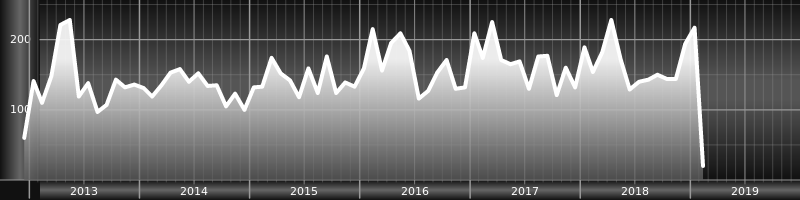
\includegraphics[width=0.5\linewidth]{images/CTAN}}%
  {Caption below with a width of the given object which may be a problem
  if it is a very small object.}{fig:width4}
\end{lstlisting}

\hvFloat[floatPos=!htb,capWidth=w]{figure}{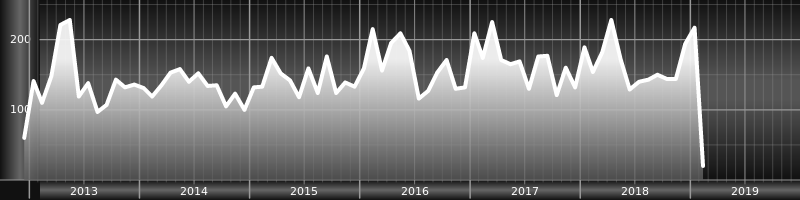
\includegraphics[width=0.5\linewidth]{images/CTAN}}%
  {Caption below with a width of the given object which may be a problem
  if it is a very small object.}{fig:width4}


\subsection{caption width to height of the object}

With \Lkeyset{capWidth=h} the caption width is like the object height which makes only
real sense if you want to put a rotated caption beside the object.

\begin{lstlisting}
\hvFloat[floatPos=!htb,capPos=after,capWidth=h,capAngle=90,objectFrame]{figure}{
\includegraphics{images/rose}}%
  {Caption beside with a width of the given object height which may be a problem
  if it is a very small object.}{fig:width5}
\end{lstlisting}

\marginnote{Fig.~\ref{fig:width5}}
\hvFloat[floatPos=!htb,capPos=after,capWidth=h,capAngle=90,objectFrame]{figure}{
\includegraphics{images/rose}}%
  {Caption beside with a width of the given object height which may be a problem
  if it is a very small object.}{fig:width5}



\section{Caption left or right of the object}
By default the caption is set on the left side of the object. If the caption and the object are set side by side, then
the keyvalue \Lkeyval{before} is identical to the setting \Lkeyval{left}.

\subsection{Caption right with specific length}
Code for figure \ref{fig:1}:
\begin{lstlisting}
\hvFloat%
  [floatPos=htb,
   capPos=right,
   objectFrame,
   objectPos=c]{figure}{
\includegraphics[scale=0.9]{images/rose}}%
  [Caption beside object and vertically centered]%
  {Caption vertically centered right beside the float with a natural caption width 
   (the default). \blindtext}%
  {fig:1}
\end{lstlisting}

\marginnote{Fig.~\ref{fig:1}}
\Float[capPos=right]
\hvFloat%
  [floatPos=htb,
   capPos=right,
   objectFrame,
   objectPos=c]{figure}{
\includegraphics[scale=0.9]{images/rose}}%
  [Caption beside object and vertically centered]%
  {Caption vertically centered right beside the float with a natural caption width 
   (the default). \hvblindtext}%
  {fig:1}


\subsection{Caption left and rotated}

Code for figure \ref{fig:2}:
\begin{lstlisting}
\hvFloat%
  [floatPos=htb,
   capPos=left,
   capWidth=h,% of \columnwidth
   capAngle=90,
   objectFrame
  ]{figure}{
\includegraphics{images/rose}}%
  [Centered Caption beside Object]%
  {Caption vertically centered left beside the float with a caption width 
   of \texttt{capWidth=h}, which is the height of the object.}{fig:2}
\end{lstlisting}

\marginnote{Fig.~\ref{fig:2}}
\hvFloat%
  [floatPos=htb,
   capPos=left,
   capWidth=h,% of \columnwidth
   capAngle=90,
   objectFrame
  ]{figure}{
\includegraphics{images/rose}}%
  [Centered Caption beside Object]%
  {Caption vertically centered left beside the float with a caption width 
   of \texttt{capWidth=h}, which is the height of the object.}{fig:2}

It is no problem to rotate the object, too. But with a different angle value than for the caption. 
Do not ask for the sense, it is only a demonstration of what is possible \ldots\  The object (image) 
is rotated by $-30$ degrees with the macro \Lcs{rotatebox}. Without any definition the caption will be
placed vertically centered to the object. Important for the height of the object is the surrounding
orthogonal rectangle.


\hvblindtext

Code for figure \ref{fig:3}:
\begin{lstlisting}
\hvFloat[%
	capWidth=h,
	capPos=after,
	capAngle=180,
	objectAngle=90,
	capVPos=center,
	objectPos=center]{figure}{\frame{
\includegraphics{images/rose}}}%
	[Centered Caption beside Object]{%
	{Caption vertically centered right beside the float with a caption width of the height 
	 of the image and a rotation of the caption and the object.}{fig:3}
\end{lstlisting}

\marginnote{Fig.~\ref{fig:3}}
\hvFloat[%
	capWidth=h,% of \columnwidth
	capPos=after,
	capAngle=180,
	objectAngle=90,
	capVPos=center,
	objectPos=center]{figure}{\frame{
\includegraphics{images/rose}}}%
  {Caption vertically centered right beside the float with a caption width of the height of the image and 
   a rotation of the caption and the object.}{fig:3}


\section{Caption inner or outer}
Setting the caption position to \emph{inner} or \emph{outer} makes only sense for a document in \Index{twoside} mode.
For a oneside document \emph{inner} is the same as \emph{left} and \emph{outer} is
the same as \emph{right}.  We show only the code for the first image with the setting \Lkeyset{capPos=inner}, 
whereas the second one
chooses only  \Lkeyset{capPos=outer}.


Code for figure~\ref{fig:20}:
\begin{lstlisting}
\hvFloat[capPos=inner]{figure}{
\includegraphics{images/rose}}%
	[Centered Caption on the inner side]{%
	Caption set with the parameter setting \texttt{capPos=inner}, which will be
	a caption on the right side for an even page and on the left side for
	an odd page.}{fig:20}
\end{lstlisting}

\marginnote{Fig.~\ref{fig:20}}
\hvFloat[capPos=inner]{figure}{
\includegraphics{images/rose}}%
	[Centered Caption on the inner side]{%
	Caption set with the parameter setting \texttt{capPos=inner}, which will be
	a caption on the right side for an even page and on the left side for
	an odd page.}{fig:20}

\hvblindtext


\label{page:1}\checkoddpage
Now the same Image with \Lkeyset{capPos=outer}. The current pagenumber is~\pageref{page:1}, an \ifoddpage odd \else
even \fi page. We now set a pagebreak at the end of the second image to see if it works with 
\emph{inner}/\emph{outer}.




\begin{lstlisting}
\hvFloat[capPos=outer]{figure}{
\includegraphics{images/rose}}%
	[Centered Caption on the inner side]{%
	Caption set with the parameter setting \texttt{capPos=outer}, which will be
	a caption on the right side for an even page and on the left side for
	an odd page.}{fig:20b}
\end{lstlisting}

\marginnote{Fig.~\ref{fig:20b}}
\hvFloat[capPos=outer]{figure}{
\includegraphics{images/rose}}%
	[Centered Caption on the inner side]{%
	Caption set with the parameter setting \texttt{capPos=outer}, which will be
	a caption on the right side for an even page and on the left side for
	an odd page.}{fig:20b}



\marginnote{Fig.~\ref{fig:21}}
\hvFloat[%
	capWidth=0.5,% of \columnwidth
	capPos=outer,
	capAngle=0,%
	capVPos=bottom,%
	objectPos=center]{figure}{
\includegraphics{images/rose}}%
	[Centered Caption beside Object]{%
	Caption at the bottom right beside the float with a caption width 
    of \texttt{0.5\textbackslash columnwidth} and and \texttt{capPos=outer}.}{fig:21}

We have an \checkoddpage
\ifoddpage odd \else
even \fi page, the reason why figure~\ref{fig:20b} has the caption for \emph{inner} on the left side
and figure~\ref{fig:21} for \emph{outer} on the right side.


\hvblindtext

\label{page:2}
Code for figure \ref{fig:22}:
\begin{lstlisting}
\hvFloat[%
	capWidth=0.5,% of \columnwidth
	capPos=inner,%  ====> INNER
	capAngle=0,
	capVPos=bottom,
	objectPos=center]{figure}{
\includegraphics{images/rose}}%
	[Centered Caption beside Object]{%
	Caption vertically centered right beside the float with a caption 
   width of \texttt{0.5\textbackslash columnwidth} and \texttt{capPos=outer} }{fig:22}
\end{lstlisting}

\marginnote{Fig.~\ref{fig:22}}
\hvFloat[%
	capWidth=0.5,% of \columnwidth
	capPos=inner,
	capAngle=0,%
	capVPos=center,%
	objectPos=center]{figure}{
\includegraphics{images/rose}}%
	[Centered Caption beside Object]{%
	Caption vertically centered right beside the float with a caption 
width of \texttt{0.5\textbackslash columnwidth} and \texttt{capPos=outer}}{fig:22}



We have an \checkoddpage
\ifoddpage odd \else
even \fi page, the reason why figure~\ref{fig:20} has the caption for \emph{inner} on the right side
and figure~\ref{fig:21} for \emph{outer} on the left side.


\section{Vertical Position of the Caption}
The caption can be placed beside the object in the positions 
\begin{verbatim}
(c)enter|(b)ottom|(t)op
\end{verbatim}

The code for figure \ref{fig:4}:
\begin{lstlisting}
\hvFloat[%
	floatPos=htb,%
	capWidth=0.25,%
	capPos=right,%
	capVPos=bottom,%
]{figure}{\frame{
\includegraphics{images/rose}}}{Caption at bottom right beside the float}{fig:4}
\end{lstlisting}


\marginnote{Fig.~\ref{fig:4}}
\hvFloat[%
	floatPos=htb,%
	capWidth=0.25,%
	capPos=right,%
	capVPos=bottom,%
]{figure}{\frame{
\includegraphics{images/rose}}}{Caption at bottom right beside the float}{fig:4}



The code for figure \ref{fig:5}:
\begin{lstlisting}
\hvFloat[%
	floatPos=htb,
	capWidth=0.25,
	capPos=right,
	capVPos=top,
]{figure}{\frame{
\includegraphics{images/rose}}}{Caption at top left beside the float}{fig:5}
\end{lstlisting}


\marginnote{Fig.~\ref{fig:5}}
\hvFloat[%
	floatPos=htb,%
	capWidth=0.25,%
	capPos=before,%
	capVPos=top,%
]{figure}{\frame{
\includegraphics{images/rose}}}{Caption at top left beside the float}{fig:5}


The code for figure \ref{fig:6}:
\begin{lstlisting}
\hvFloat[%
	capWidth=0.25,%
	capPos=right,%
	capVPos=center,% the default
]{figure}{\frame{
\includegraphics{images/rose}}
          \frame{
\includegraphics[origin=c,angle=180]{images/rose}}}%
 {Caption centered right beside the float}{fig:6}
\end{lstlisting}


\marginnote{Fig.~\ref{fig:6}}
\hvFloat[%
	capWidth=0.25,%
	capPos=right,%
	capVPos=center,% the default
]{figure}{\frame{
\includegraphics{images/rose}}
          \frame{
\includegraphics[origin=c,angle=180]{images/rose}}}%
 {Caption centered right beside the float}{fig:6}


\section{Caption format}
The \Lcs{caption} and \Lcs{subcaption} macros are fully under the control of the package \Lpack{caption}.
The formatting can be set with the macros \Lcs{captionsetup}, \Lcs{subcaptionsetup}, or via the optional
argument setting of \Lcs{hvFloat} with the keywords \Lkeyword{capFormat}  and \Lkeyword{subcapFormat}.
The argument itself will then be used internally by \Lcs{captionsetup} and/or \Lcs{subcaptionsetup}
in a minipage, the reason why it will be local to the current image..

\begin{lstlisting}
\hvFloat[%
  capPos=right,
  capFormat={labelsep=newline,justification=RaggedRight,font={small,it},labelfont=bf}
]{figure}{\frame{
\includegraphics{images/rose}}}{\blindtext}{fig:66}
\end{lstlisting}

\marginnote{Fig.~\ref{fig:66}}
\hvFloat[%
  capPos=right,
  capFormat={labelsep=newline,justification=RaggedRight,font={small,it},labelfont=bf}
]{figure}{\frame{
\includegraphics{images/rose}}}{\hvblindtext}{fig:66}


\section{Horizontal Position of the Float}

The caption is always near the object, only divided by the length \Ldim{floatCapSep}
which can be set by the keyword of the same name \Lkeyword{floatCapSep}. It accepts only
a value with any allowed unit. %The default unit is \texttt{pt} and cannot be changed.
The keyword \Lkeyword{objectPos} refers always to the complete floating object: caption 
\emph{and} object. The meaning of \Lkeyset{objectPos=left} is: Put the object as far as possible to the
left margin. If \Lkeyset{capPos=left} is also used, then the caption is at the left margin followed by
the object (see Figure~\vref{fig:700}).

The code for figure \ref{fig:7}:
\begin{lstlisting}
\hvFloat[%
	capWidth=0.25,
	capPos=right,
	capVPos=top,
	objectPos=left,
	objectFrame,
]{figure}{
\includegraphics{images/rose}}{%
	Caption at top right beside the float and object position left}{fig:7}
\end{lstlisting}


\marginnote{Fig.~\ref{fig:7}}
\hvFloat[%
	capWidth=0.25,%
	capPos=right,%
	capVPos=top,%
	objectPos=left,%
	objectFrame,
]{figure}{
\includegraphics{images/rose}}{%
	Caption at top right beside the float and object position left}{fig:7}

\hvblindtext


The same with \Lkeyset{capPos=left}:


\marginnote{Fig.~\ref{fig:700}}
\hvFloat[%
	capWidth=0.25,%
	capPos=left,%
	capVPos=top,%
	objectPos=left,%
	objectFrame,
]{figure}{
\includegraphics{images/rose}}{%
	Caption at top right beside the float and object position left}{fig:700}

\hvblindtext


The code for figure \ref{fig:8}:
\begin{lstlisting}
\hvFloat[%
	capWidth=0.25,
	capPos=before,
	capVPos=top,
	objectPos=right,
	objectFrame,
]{figure}{
\includegraphics{images/rose}}{%
	Caption at top leftt beside the float and object position right}{fig:8}
\end{lstlisting}


\marginnote{Fig.~\ref{fig:8}}
\hvFloat[%
	capWidth=0.25,%
	capPos=before,%
	capVPos=top,%
	objectPos=right,%
	objectFrame,
]{figure}{
\includegraphics{images/rose}}{%
	Caption at top left beside the float and object position right}{fig:8}

\hvblindtext


\section{Wide floats}

With the optional argument \Lkeyword{wide} the width of the defined \Ldim{marginparwidth} is
added to the allowed horizontal width of the float.

The code for figure \ref{fig:70}:
\begin{lstlisting}
\hvFloat[wide,
	capPos=right,
	capVPos=top,
	objectPos=left,
]{figure}{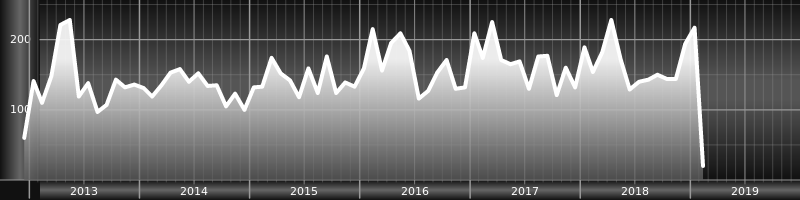
\includegraphics[width=0.75\linewidth]{images/CTAN}}{%
	Caption at top right beside the float and object position left and
the option \texttt{wide}.}{fig:70}
\end{lstlisting}

\marginnote{Fig.~\ref{fig:70}}
\hvFloat[%
	wide,
	capPos=right,%
	capVPos=top,%
	objectPos=left,%
]{figure}{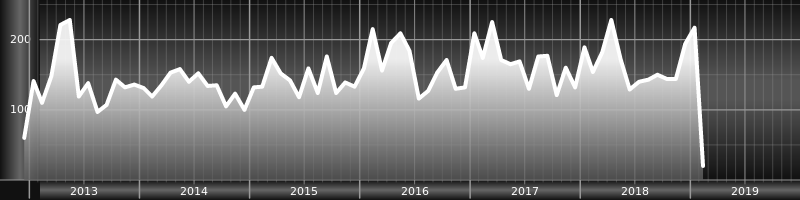
\includegraphics[width=0.75\linewidth]{images/CTAN}}{%
	Caption at top right beside the float and object position left and
the option \texttt{wide}.}{fig:70}

%\hvblindtext


The code for figure \ref{fig:80}:
\begin{lstlisting}
\hvFloat[wide,
	capPos=left,
	capVPos=top,
	objectPos=right,
  ]{figure}{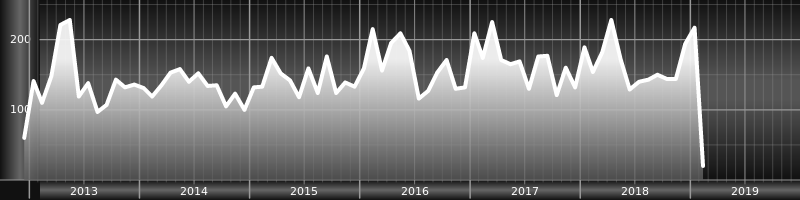
\includegraphics[width=0.75\linewidth]{images/CTAN}}%
  {Caption at top left beside the object and object position left and
   the option \texttt{wide}.}{fig:80}
\end{lstlisting}


\marginnote{Fig.~\ref{fig:80}}
\hvFloat[wide,
	capPos=left,%
	capVPos=top,%
]{figure}{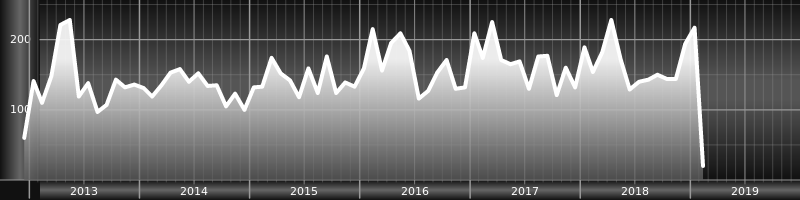
\includegraphics[width=0.75\linewidth]{images/CTAN}}%
  {Caption at top left beside the object and object position left and
   the option \texttt{wide}.}{fig:80}


For a twosided document it will place the object always in the margin.

\hvblindtext

\begin{lstlisting}
\hvFloat[wide,
	capPos=inner,
	capVPos=top,
]{figure}{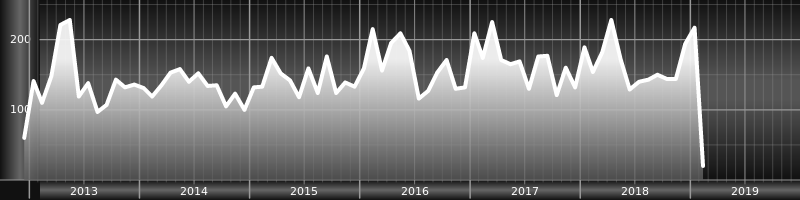
\includegraphics[width=0.75\linewidth]{images/CTAN}}{%
Caption at top and inner beside the float and object position right and
the option \texttt{wide}.}{fig:81}
\end{lstlisting}

\marginnote{Fig.~\ref{fig:81}}
\hvFloat[wide,
	capPos=inner,
	capVPos=top,
]{figure}{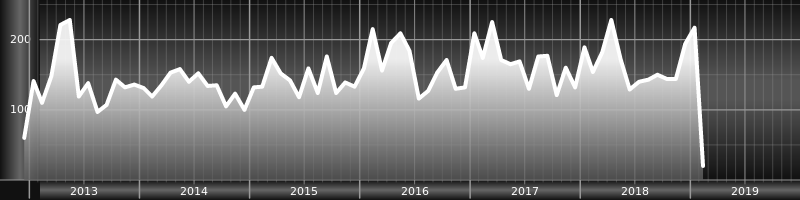
\includegraphics[width=0.75\linewidth]{images/CTAN}}{%
Caption at top and inner beside the float and object position right and
the option \texttt{wide}.}{fig:81}

Now we set the same image with the same setting on the next page. The caption will
change its side due to the setting \Lkeyset{capPos=outer}.

\hvblindtext



\begin{lstlisting}
\hvFloat[wide,
	capPos=inner,
	capVPos=top,
]{figure}{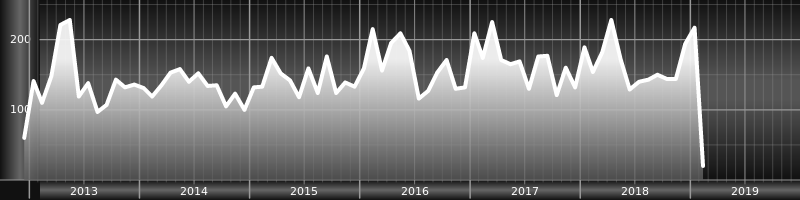
\includegraphics[width=0.75\linewidth]{images/CTAN}}{%
Caption at top inner beside the float and object position right and
the option \texttt{wide}.}{fig:811}
\end{lstlisting}


\marginnote{Fig.~\ref{fig:811}}
\hvFloat[wide,
	capPos=inner,
	capVPos=top,
]{figure}{\includegraphics[width=0.75\linewidth]{images/CTAN}}{%
Caption at top inner beside the float and object position right and
the option \texttt{wide}.}{fig:811}

The caption can be typeset completely into the margin with:

\begin{lstlisting}
\captionsetup{justification=RaggedRight}
\hvFloat[wide,
	capPos=outer,
	capVPos=top,
        floatCapSep=\marginparsep,
]{figure}{\includegraphics[width=\linewidth]{images/CTAN}}{%
Caption at top inner beside the float and object position right and
the option \texttt{wide}.}{fig:812}
\end{lstlisting}

%\Float[capPos=outer]

\begingroup
\marginnote{Fig.~\ref{fig:812}}
\captionsetup{justification=RaggedRight}
\hvFloat[wide,
	capPos=outer,
	capVPos=top,
        floatCapSep=\marginparsep,
]{figure}{\includegraphics[width=\linewidth]{images/CTAN}}{%
Caption at top inner beside the float and object position right and
the option \texttt{wide}.}{fig:812}
\endgroup



\section{The star version \Lcs{hvFloat*}}\label{star-version0}
In the \Index{twocolumn} mode the floating environment can be set over both
columns with the star version \Lcs{hvFloat*}. The floating environment will
not be on the bottom of the page. The code for 
the following example (Figure~\vref{default1s2c}) is:

\begin{lstlisting}
\hvFloat*[capPos=right]{figure}%
  {\includegraphics{images/frose}}%
  [A  float with the default caption setting]%
  {A default caption of a ``'' object with the default setting, which
   is a ``left''  caption which means that it always appears before the object.
   This can be an even or odd page. And some more text whch has no
   real meaning because it fills only the space for a long caption.}%
  {fig:0}
\end{lstlisting}

The example shows on page 3 the star version and on page 4 the same without using the star.


\begin{figure}[!h]
\frame{\includegraphics[page=2,width=0.24\linewidth]{examples/default1s2c}}\hfill
\frame{\includegraphics[page=3,width=0.24\linewidth]{examples/default1s2c}}\hfill
\frame{\includegraphics[page=4,width=0.24\linewidth]{examples/default1s2c}}\hfill
\frame{\includegraphics[page=5,width=0.24\linewidth]{examples/default1s2c}}
\caption{Output of \texttt{default1s2c} (pages 2 --5)}\label{default1s2c}
\end{figure}




\section{Full Page Width in Landscape Mode}

If you do not want to load the package \Lpack{lscape} (or \Lpack{pdflscape}) you can use the \Lkeyset{floatPos=p} 
option to put the image on an own page and rotated by 90 degrees (figure~\ref{fig:9}). 




Code for figure \ref{fig:9}:
\begin{lstlisting}
\hvFloat[%
	floatPos=p,
	capPos=bottom,
	rotAngle=90,
	objectPos=center,
]{figure}{\includegraphics[width=0.9\textheight]{images/CTAN}}%
  [Object and Caption in landscape mode]{%
	Caption and object in landscape mode. \blindtext}{fig:9}
\end{lstlisting}

The float can also be put to the left or to the right  (above/below in landscape) 
with the \Lkeyset{objectPos=l} parameter

\marginnote{Fig.~\ref{fig:9}}
\hvFloat[%
	floatPos=p,
	capPos=bottom,
	rotAngle=90,
	objectPos=center,
]{figure}{\includegraphics[width=0.9\textheight]{images/CTAN}}%
  [Object and Caption in landscape mode]{%
	Caption and object in landscape mode. \hvblindtext}{fig:9}


\hvblindtext


The code for figure \ref{fig:10}:
\begin{lstlisting}
\hvFloat[%
	floatPos=p,
	capWidth=h,
	capPos=right,
	objectAngle=90,
	capAngle=-90,
	objectPos=left,
]{figure}{\includegraphics[width=\textheight]{images/CTAN}}%
	[Rotated Caption in Landscape]{%
	Caption right beside the float and object position left. The caption rotated by $-90$ 
        degrees.\blindtext}{fig:10}
\end{lstlisting}

\marginnote{Fig.~\ref{fig:10}}
\hvFloat[%
	floatPos=p,%
	capWidth=h,%
	capPos=right,%
	objectAngle=90,%
	capAngle=-90,%
	objectPos=left%
]{figure}{\includegraphics[width=\textheight]{images/CTAN}}%
	[Rotated Caption in Landscape]{%
	Caption right beside the float and object position left. The caption rotated by $-90$ degrees.
        \hvblindtext}{fig:10}



\hvblindtext

\hvblindtext



\section{The \Lkeyword{nonFloat} Option}
Sometimes it is better to put a ``float'' in a specific position of the page. This is possible 
with the \Lpack{nonfloat} package and the keyword \Lkeyword{nonFloat}. 

\begin{lstlisting}
Some nonsense text before the following \emph{non floating} object.

\hvFloat[%
	nonFloat,
	capWidth=0.25,
	capPos=right,
	capVPos=bottom,
	objectPos=center,
	objectFrame,
]{figure}{\includegraphics[scale=1.5]{images/rose}}%
	[Nonfloat Captions]{%
	Caption of a ``nonfloat'' Object, using the \texttt{nonfloat} Package}{fig:11}

Some nonsense text after the preceding  \emph{non floating} object.
\end{lstlisting}

Some nonsense text before the following \emph{non floating} object.

\marginnote{Fig.~\ref{fig:11}}
\hvFloat[%
	nonFloat,%
	capWidth=0.25,%
	capPos=right,%
	capVPos=bottom,%
	objectPos=center,%
        objectFrame,
]{figure}{\includegraphics[scale=1.5]{images/rose}}%
	[Nonfloat Captions]{%
	Caption of a ``nonfloat'' Object, using the \texttt{nonfloat} Package}{fig:11}

Some nonsense text after the preceding  \emph{non floating} object.

\bigskip
The image \ref{fig:11} is exactly placed where the command \Lcs{hvFloat} appears. 
There are only commands for \Lenv{figure} and \Lenv{table} environments:

\begin{verbatim}
\newcommand{\figcaption}{\def\@captype{figure}\caption}
\newcommand{\tabcaption}{\def\@captype{table}\caption}
\end{verbatim}

But it is no problem, to define more \texttt{xxxcaption} commands to support other with the 
\Lpack{float} package defined new floats.





\section{Tabulars as Objects}\label{sec:tables}
The object has to be passed as an parameter to the \Lcs{hvFloat} macro. This is no 
problem with images but maybe with tables, so it is easier to use the box \Lcs{hvOBox} 
to save the table in this box and pass it then to \Lcs{hvFloat} with the \Lkeyword{useOBox} option. 
For example see table~\ref{table:1} and \ref{table:2}:

\savebox{\hvOBox}{%
 \begin{tabular}{>{\small\ttfamily}l|l|l}\hline
  \rmfamily Name    & Type        & Description\\\hline
  \CMD{hvFloat}  & command     & places object and caption in different ways\\
  hvFloatEnv  & environment & places object and caption exactly Here\\
  \CMD{figcaption} & command   & writes a figure caption in a non floating environment\\
  \CMD{tabcaption} & command   & writes a table caption in a non floating environment\\
  \CMD{hvFloatSetDefaults} & command  & sets all options to the defaults\\\hline
 \end{tabular}%
}

\hvblindtext

%[xrightmargin=-8em,xleftmargin=-1em]
\begin{lstlisting}
\savebox{\hvOBox}{%
 \begin{tabular}{>{\small\ttfamily}l|l|l}\hline
  \rmfamily Name    & Type        & Description\\\hline
  \CMD{hvFloat}  & command     & places object and caption in different ways\\
  hvFloatEnv  & environment & places object and caption exactly Here\\
  \CMD{figcaption} & command   & writes a figure caption in a non floating environment\\
  \CMD{tabcaption} & command   & writes a table caption in a non floating environment\\
  \CMD{hvFloatSetDefaults} & command  & sets all options to the defaults\\\hline
 \end{tabular}%
}
\end{lstlisting}

The code for table \ref{table:1} and \ref{table:2} is: 

%[xrightmargin=-7em,xleftmargin=-3em]
\begin{lstlisting}
\hvFloat[%
  floatPos=!hb,
  capPos=top,
  useOBox=true]{table}{}{Demonstration of the \texttt{useOBox} Parameter}{table:1}

\hvblindtext

\marginnote{Tab.~\ref{table:2}}
\hvFloat[%
  floatPos=hb,
  useOBox=true,
  objectAngle=90,
  capPos=right,
  capVPos=top,
  capWidth=0.3]{table}{}{Another demonstration of the \texttt{useOBox} Parameter}{table:2}
\end{lstlisting}

In this case leave the third parameter empty.

\marginnote{Tab.~\ref{table:1}}
\hvFloat[%
  floatPos=!hb,
  capPos=top,
  useOBox=true]{table}{}{Demonstration of the \texttt{useOBox} Parameter}{table:1}



\marginnote{Tab.~\ref{table:2}}
\hvFloat[%
	floatPos=!htb,%
	useOBox=true,%
	objectAngle=90,%
	capPos=right,%
	capVPos=top,%
	capWidth=0.3]{table}{}{Demonstration of the \texttt{useOBox} Parameter}{table:2}


\section{Text and objects}\label{sec:text}

With the \Lkeyword{onlyText} keyword it is no problem to put some text beside an image without 
getting the caption title Figure/Table. The object still can be a floating one or a nonfloating 
if the \Lkeyword{nonfloat} keyword is used.

The code for figure \ref{fig:text}:

\begin{lstlisting}
\hvFloat[%
  onlyText=true,
  capAngle=90,
  capPos=right,
  capVPos=top,
  objectFrame,
  capWidth=h]{}{\includegraphics{images/rose}}%
  [``\texttt{onlyText}'' Caption]{%
    Demonstration of the \texttt{onlyText} Parameter, which makes it 
    possible to put some text beside a floating object without getting 
    a starting \texttt{Figure:} or \texttt{Table:}}{fig:text}
\end{lstlisting}


\marginnote{Fig.~\ref{fig:text}}
\hvFloat[%
	onlyText=true,%
	capAngle=90,%
	capPos=right,%
	capVPos=top,%
	objectFrame,
	capWidth=h]{}{\includegraphics{images/rose}}%
	[``\texttt{onlyText}'' Caption]{%
	Demonstration of the \texttt{onlyText} Parameter, which makes it 
	possible to put some text beside a floating object without getting 
	a starting \texttt{Figure:} or \texttt{Table:}}{fig:text}

\bigskip
%\hvblindtext

%\hvblindtext

\section{Environment \texttt{hvFloatEnv}}\label{sec:env}

With the environment \Lenv{hvFloatEnv} one can place an object exactly on that position where the
environment is defined. For captions the use of \Lcs{captionof} is recommended:

\begin{lstlisting}
\begin{hvFloatEnv}
\captionof{table}{A caption for a nice table}
\begin{tabular}{@{} l c r @{}}\hline
left & center & right \\
L    & C      & R     \\\hline
\end{tabular}
\end{hvFloatEnv}
\end{lstlisting}

\begin{hvFloatEnv}
\captionof{table}{A caption for a nice table}
\begin{tabular}{@{} l c r @{}}\hline
left & center & right \\
L    & C      & R     \\\hline
\end{tabular}
\end{hvFloatEnv}


\bigskip
The environment has an optional argument for setting the line width which is preset to \Ldim{textwidth}.
The object is always centered.


\begin{lstlisting}
\begin{hvFloatEnv}[0.5\textwidth]
\captionof{table}{A caption for a nice table}
\begin{tabular}{@{} l c r @{}}\hline
left & center & right \\
L    & C      & R     \\\hline
\end{tabular}
\end{hvFloatEnv}
\end{lstlisting}


\begin{hvFloatEnv}[0.5\textwidth]
\captionof{table}{A caption for a nice table}
\begin{tabular}{@{} l c r @{}}\hline
left & center & right \\
L    & C      & R     \\\hline
\end{tabular}
\end{hvFloatEnv}

%\bigskip
%\hvblindtext

%\hvblindtext


\section{Full page objects in onecolumn mode}
For an image or table which needs the whole space of a page the caption can be 
printed at the bottom of the preceeding or following page. It is possible in
oneside and twoside mode, but makes only real sense in the twoside mode.
%
\Lpack{hvfloat} defines three additional optional arguments for placing
images in a complete column, page or paper:

\noindent
\minipage[t]{0.49\linewidth}
\begin{verbatim}
\define@key{Gin}{fullpage}[true]{%
  \def\Gin@ewidth{\columnwidth}%
  \def\Gin@eheight{\textheight}%
  \Gin@boolkey{false}{iso}%
}
\define@key{Gin}{FULLPAGE}[true]{%
  \def\Gin@ewidth{\paperwidth}%
  \def\Gin@eheight{\paperheight}%
  \Gin@boolkey{false}{iso}%
}
\end{verbatim}
\endminipage\hfill
\minipage[t]{0.49\linewidth}
\begin{verbatim}
\define@key{Gin}{FullPage}[true]{%
  \def\Gin@ewidth{\textwidth}%
  \def\Gin@eheight{\textheight}%
  \Gin@boolkey{false}{iso}%
}
\end{verbatim}
\endminipage

Figure~\vref{fig:fullpage60} shows the meaning of the optional arguments \Lkeyword{fullpage}, 
\Lkeyword{FullPage}, and \Lkeyword{FULLPAGE} for \Lcs{inclugegraphics}\OptArg{...}\Largb{tiger}.

\begin{figure}[!h]
\frame{\includegraphics[page=1,width=0.24\linewidth]{examples/fullpage1s2c}}\hfill
\frame{\includegraphics[page=2,width=0.24\linewidth]{examples/fullpage1s2c}}\hfill
\frame{\includegraphics[page=3,width=0.24\linewidth]{examples/fullpage1s2c}}\hfill
\frame{\includegraphics[page=4,width=0.24\linewidth]{examples/fullpage1s2c}}

\frame{\includegraphics[page=5,width=0.24\linewidth]{examples/fullpage1s2c}}\hfill
\frame{\includegraphics[page=6,width=0.24\linewidth]{examples/fullpage1s2c}}\hfill
\frame{\includegraphics[page=7,width=0.24\linewidth]{examples/fullpage1s2c}}\hfill
\frame{\includegraphics[page=8,width=0.24\linewidth]{examples/fullpage1s2c}}
\caption{Output of \texttt{fullpage1s2c} (pages 1--8)}\label{fig:fullpage60}
\end{figure}





\subsection{Using the textarea}

The setting \Lkeyset{capPos=evenPage} (even) or \Lkeyset{capPos=oddPage} (odd) page for
a document in \Index{twocolumn} mode makes no real sense. For a twosided document a 
setting like \Lkeyset{capPos=inner} for inner or \Lkeyset{capPos=outer} for outer
margin makes more sense.
%
For an image or table which needs the whole space of a page the caption can be 
printed at the bottom of the preceeding or following page. It is possible in
oneside and twoside mode, but makes only real sense in the twoside mode.
Without any additional argument the caption is set first and the object on the follwing page:



\subsubsection{Using the default or \Lkeyset{capPos=before}}

Without any additional argument the caption is set first (left) at the bottom of the current page 
and the object on the following page. This is the same setting like \Lkeyset{capPos=left} for a onecolumn document.
For the \Loption{twocolumn} option it makes more sense to use the setting \Lkeyset{capPos=before} if the
caption and object can appear on different pages.




\begin{lstlisting}
\hvFloat[fullpage]%
  {figure}%
  {\includegraphics[fullpage]{images/frose}}%
  [A fullpage float with the default caption setting]%
  {A default caption of a ``fullpage'' object with the default setting, which
   is a ``left''  caption which means that it always appears ``before'' the object.
   This can be an even or odd page. And some more text whch has no
   real meaning because it fills only the space for a long caption.}%
  {fig:fullpage0}
\end{lstlisting}






\begin{table}[!h]
\caption{Valid optional arguments for a full page object.}\label{tab:fullpage}
\centering
 \begin{tabularx}{\linewidth}{>{\small\ttfamily}l|>{\small\ttfamily}l|X}\toprule
  \rmfamily Name    & \rmfamily Type        & Description\\\midrule
\Lkeyword{fullpage} & true|false & Put the caption on the bottom of the preceding or following page and the object alone a page.\\

%\Lkeyword{FullPage} & true|false & The same for \Index{twocolumn} mode with object over both columns.\\

\Lkeyword{FULLPAGE} & true|false & The same for full papersize objects over one or two columns. 
The pagestyle is set to \texttt{empty}\\

\Lkeyword{multiFloat} & true|false & For multiple objects with captions for every object. See section~\vref{sec:multifloats}.\\

\Lkeyword{subFloat} & true|false & For multiple objects with one main and more subcaptions. See section~\vref{sec:subfloats}.\\

\Lkeyword{separatorLine} & true & Put a line with a predefined width of 0.4pt between
    the text and the caption. Only valid for the keyword \Lkeyword{fullpage}.\\
\Lkeyword{capPos}  & value
	 & caption \Lkeyval{before}, \Lkeyval{after} an object or on an
		    \Lkeyval{evenPage} or \Lkeyval{oddPage}.\\
\bottomrule
 \end{tabularx}%
\end{table}




With this setting the caption is always placed \textit{before} the following object. 
This maybe sufficient for a \Index{oneside} document but  not the best solution if
this document is printed on a duplex machine. In such a case
it may make sense to have the captions always on an even (left) page, even though the
socument is typeset in a oneside mode. Figure~\vref{fig:fullpage0} shows the output
for a oneside document with a setting \Lkeyset{capPos=before}.



Depending to the
used documentclass it can be a problem, if the caption should be placed on the first page.
In such a case use one of the other setting.
Table~\vref{tab:fullpage} shows the valid optional arguments for a full page floating object.




\begin{figure}[!h]
\frame{\includegraphics[page=2,width=0.24\linewidth]{examples/default1s1c}}\hfill
\frame{\includegraphics[page=3,width=0.24\linewidth]{examples/default1s1c}}\hfill
\frame{\includegraphics[page=4,width=0.24\linewidth]{examples/default1s1c}}\hfill
\frame{\includegraphics[page=5,width=0.24\linewidth]{examples/default1s1c}}

\frame{\includegraphics[page=6,width=0.24\linewidth]{examples/default1s1c}}\hfill
\frame{\includegraphics[page=7,width=0.24\linewidth]{examples/default1s1c}}\hfill
\frame{\includegraphics[page=8,width=0.24\linewidth]{examples/default1s1c}}\hfill
\frame{\includegraphics[page=9,width=0.24\linewidth]{examples/default1s1c}}
\caption{Output of \texttt{default1s1c} (pages 2--9)}\label{fig:fullpage0}
\end{figure}






%\FloatBarrier

\clearpage

\subsubsection{Using \Lkeyset{capPos=after}}

The  caption will be printed always on the right side which is the same as \textit{after} the full page object.
The object appers immediately on the next page and the caption of the next following page at the bottom. There
is no check for an even or odd page. This behaviour makes only sense for a oneside document. 

\begin{lstlisting}
\hvFloat[fullpage, capPos=after]%
  {figure}%
  {\includegraphics[fullpage]{images/frose}}%
  [A float which needs the complete page width and height.]%
  {A Caption of a ``fullpage'' object, which follows on the next page. 
   This can be an even or odd page. And some more text whch has no
   real meaning because it fills only the space for a long caption.}
  {fig:fullpage1}
\end{lstlisting}



\begin{figure}[!h]
\frame{\includegraphics[page=2,width=0.24\linewidth]{examples/after1s1c}}\hfill
\frame{\includegraphics[page=3,width=0.24\linewidth]{examples/after1s1c}}\hfill
\frame{\includegraphics[page=4,width=0.24\linewidth]{examples/after1s1c}}\hfill
\frame{\includegraphics[page=5,width=0.24\linewidth]{examples/after1s1c}}

\frame{\includegraphics[page=6,width=0.24\linewidth]{examples/after1s1c}}\hfill
\frame{\includegraphics[page=7,width=0.24\linewidth]{examples/after1s1c}}\hfill
\frame{\includegraphics[page=8,width=0.24\linewidth]{examples/after1s1c}}\hfill
\frame{\includegraphics[page=9,width=0.24\linewidth]{examples/after1s1c}}
\caption{Output of \texttt{after1s1c} (pages 2--9)}\label{after1s1c}
\end{figure}


%\FloatBarrier

\clearpage

\subsubsection{Using \Lkeyset{capPos=evenPage} --- caption on an even page}

With \Lkeyset{capPos=evenPage} the caption will be printed on an even (left) page, 
the object will always be on an odd (right) page.
This option makes only real sense for The \Loption{twoside} mode!


\begin{lstlisting}
\hvFloat[fullpage, capPos=evenPage]%
  {figure}%
  {\includegraphics[fullpage]{images/frose}}%
  [A float whith a caption on an even page (left)]%
  {A caption on an even (left) page of a ``fullpage'' object.. \blindtext}
  {fig:fullpage3}
\end{lstlisting}


\begin{figure}[!h]
\frame{\includegraphics[page=2,width=0.24\linewidth]{examples/even1s1c}}\hfill
\frame{\includegraphics[page=3,width=0.24\linewidth]{examples/even1s1c}}\hfill
\frame{\includegraphics[page=4,width=0.24\linewidth]{examples/even1s1c}}\hfill
\frame{\includegraphics[page=5,width=0.24\linewidth]{examples/even1s1c}}

\frame{\includegraphics[page=6,width=0.24\linewidth]{examples/even1s1c}}\hfill
\frame{\includegraphics[page=7,width=0.24\linewidth]{examples/even1s1c}}\hfill
\frame{\includegraphics[page=8,width=0.24\linewidth]{examples/even1s1c}}\hfill
\frame{\includegraphics[page=9,width=0.24\linewidth]{examples/even1s1c}}
\caption{Output of \texttt{even1s1c} (pages 2--9)}\label{fig:fullpage6}

\end{figure}


%\FloatBarrier
\clearpage


\subsubsection{Using \Lkeyset{capPos=oddPage} --- caption on an odd page}

With \Lkeyset{capPos=oddPage} the caption will be printed on an odd (right) page, the object will always be on an even (left) page,
which is before the caption.
%This option makes only sense for The \Loption{twoside} mode!


\begin{lstlisting}
\hvFloat[fullpage, capPos=oddPage]%
  {figure}%
  {\includegraphics[fullpage]{images/frose}}%
  [A float which needs the complete page width and height.]%
  {A Caption on an odd page of a ``fullpage'' object, which follows on the next page. 
   This can be an even or odd page. And some more text whch has no
   real meaning because it fills only the space for a long caption.}
  {fig:fullpage2}
\end{lstlisting}



\begin{figure}[!h]
\frame{\includegraphics[page=2,width=0.24\linewidth]{examples/odd1s1c}}\hfill
\frame{\includegraphics[page=3,width=0.24\linewidth]{examples/odd1s1c}}\hfill
\frame{\includegraphics[page=4,width=0.24\linewidth]{examples/odd1s1c}}\hfill
\frame{\includegraphics[page=5,width=0.24\linewidth]{examples/odd1s1c}}

\frame{\includegraphics[page=6,width=0.24\linewidth]{examples/odd1s1c}}\hfill
\frame{\includegraphics[page=7,width=0.24\linewidth]{examples/odd1s1c}}\hfill
\frame{\includegraphics[page=8,width=0.24\linewidth]{examples/odd1s1c}}\hfill
\frame{\includegraphics[page=9,width=0.24\linewidth]{examples/odd1s1c}}
\caption{Output of \texttt{odd1s1c} (pages 2--9)}\label{fig:fullpage10}
\end{figure}

\iffalse
\begin{figure}
\frame{\includegraphics[page=4,width=0.24\linewidth]{examples/odd2s1c}}\hfill
\frame{\includegraphics[page=5,width=0.24\linewidth]{examples/odd2s1c}}\hfill
\frame{\includegraphics[page=6,width=0.24\linewidth]{examples/odd2s1c}}\hfill
\frame{\includegraphics[page=7,width=0.24\linewidth]{examples/odd2s1c}}

\frame{\includegraphics[page=8,width=0.24\linewidth]{examples/odd2s1c}}\hfill
\frame{\includegraphics[page=9,width=0.24\linewidth]{examples/odd2s1c}}\hfill
\frame{\includegraphics[page=10,width=0.24\linewidth]{examples/odd2s1c}}\hfill
\frame{\includegraphics[page=11,width=0.24\linewidth]{examples/odd2s1c}}
\caption{Output of \texttt{odd2s1c} (pages 4--11)}\label{fig:fullpage12}
\end{figure}
\fi




\FloatBarrier


\subsubsection{Using \Lkeyset{capPos=inner} or \Lkeyset{capPos=outer}--- caption on the inner or outer side}

These settings make no sense in \Index{onecolumn} mode.


\clearpage




\subsection{Using the paper size}

It belongs to the user to create an object which fills the complete page. However, with the
keyword \Lkeyword{FULLPAGE} which is valis for \Lcs{hvfloat} \emph{and} 
for the macro \Lcs{includegraphics} an image will be scaled to
the paper dimensions \Ldim{paperwidth} and
\Ldim{paperheight}. It can be used in one- and twocolumn mode!

\begin{lstlisting}
\hvFloat[FULLPAGE]%
  {figure}%
  {\includegraphics[FULLPAGE]{frose.png}}%
  [A fullpage float with the default caption setting]%
  {A default caption of a ``fullpage'' object with the default setting, which
   is a ``left''  caption which means that it always appears before the object.
   This can be an even or odd page. And some more text whch has no
   real meaning because it fills only the space for a long caption.}%
  {fig:fullpage0}
\end{lstlisting}



\begin{figure}[!h]
\frame{\includegraphics[page=2,width=0.24\linewidth]{examples/paper-default1s1c}}\hfill
\frame{\includegraphics[page=3,width=0.24\linewidth]{examples/paper-default1s1c}}\hfill
\frame{\includegraphics[page=4,width=0.24\linewidth]{examples/paper-default1s1c}}\hfill
\frame{\includegraphics[page=5,width=0.24\linewidth]{examples/paper-default1s1c}}

\frame{\includegraphics[page=6,width=0.24\linewidth]{examples/paper-default1s1c}}\hfill
\frame{\includegraphics[page=7,width=0.24\linewidth]{examples/paper-default1s1c}}\hfill
\frame{\includegraphics[page=8,width=0.24\linewidth]{examples/paper-default1s1c}}\hfill
\frame{\includegraphics[page=9,width=0.24\linewidth]{examples/paper-default1s1c}}
%\frame{\includegraphics[page=10,width=0.24\linewidth]{examples/paper-default1s1c}}
\caption{Output of \texttt{paper-default1s1c} (pages 2--9)}\label{paper-default1s1c}
\end{figure}

\begin{figure}[!h]
\frame{\includegraphics[page=2,width=0.24\linewidth]{examples/paper-after1s1c}}\hfill
\frame{\includegraphics[page=3,width=0.24\linewidth]{examples/paper-after1s1c}}\hfill
\frame{\includegraphics[page=4,width=0.24\linewidth]{examples/paper-after1s1c}}\hfill
\frame{\includegraphics[page=5,width=0.24\linewidth]{examples/paper-after1s1c}}

\frame{\includegraphics[page=6,width=0.24\linewidth]{examples/paper-after1s1c}}\hfill
\frame{\includegraphics[page=7,width=0.24\linewidth]{examples/paper-after1s1c}}\hfill
\frame{\includegraphics[page=8,width=0.24\linewidth]{examples/paper-after1s1c}}\hfill
\frame{\includegraphics[page=9,width=0.24\linewidth]{examples/paper-after1s1c}}
%\frame{\includegraphics[page=10,width=0.24\linewidth]{examples/paper-after1s1c}}
\caption{Output of \texttt{paper-after1s1c} (pages 2--9)}\label{paper-after1s1c}
\end{figure}


\FloatBarrier


\clearpage


\subsection{Multifloats}\label{sec:multifloats}
Multifloats is the name for more than one image and/or tabular in \emph{one} floating
environment. Every image and/or tabular has its own caption, which is different to
a subcaption. The syntax for multiple floats is

\begin{BDef}
\Lcs{hvFloat}\OptArgs&+\Largb{float type}\Largb{floating object}\OptArg{short caption}\Largb{long caption}\Largb{label}\\
&+\Largb{float type}\Largb{floating object}\OptArg{short caption}\Largb{long caption}\Largb{label}\\
&+\ldots\\
&+\Largb{float type}\Largb{floating object}\OptArg{short caption}\Largb{long caption}\Largb{label}
\end{BDef}

The + symbol defines an additional Object which will be part of the same floating environment.
It's up too the user to be sure that one page or one column can hold all defined objects.
Every object gets its own caption which is the reason why figures and tabulars and \ldots\ 
can be mixed:

\begin{lstlisting}
\captionsetup{singlelinecheck=false}
\hvFloat[fullpage,capPos=before,multiFloat,vFill]%
  +{figure}{\includegraphics[width=\linewidth]{images/CTAN}}%%                   no 1
   [Short caption A]%
   {A Caption A of a ``fullpage'' object, which follows on the left or
    right column. This can be an even or odd page. And some more text whch has no
    real meaning because it fills only the space for a long caption.}%
   {img:demo0}%
  +{table}{\begin{tabular}{lrcp{3cm}}\hline                        %             no 2
            Linksbündig & Rechtsbündig & Zentriert & Parbox\\\hline
            L           & R            & C         & P\\
            left        & right        & center    & Text with possible linebreaks\\
            \multicolumn{4}{c}{Multicolumn over all columns}\\\hline
           \end{tabular}}%
   [Short Caption B]%
   {A Caption B of a ``fullpage'' object, which follows on the left or
        right column. This can be an even or odd page.}{}%
  +{figure}{\includegraphics[width=\linewidth]{images/CTAN}}%%                    no 3
   {A Caption C of a ``fullpage'' object, which follows on the left or
      right column.}%
   {img:demo1}
  +{figure}{\includegraphics[width=\linewidth]{images/CTAN}}%%                    no 4
   {A Caption C of a ``fullpage'' object, which follows on the left or
      right column.}%
   {img:demo2}
\end{lstlisting}


\begin{figure}[!h]
\frame{\includegraphics[page=4,width=0.24\linewidth]{examples/multi-default1s1c}}\hfill
\frame{\includegraphics[page=5,width=0.24\linewidth]{examples/multi-default1s1c}}\hfill
\frame{\includegraphics[page=6,width=0.24\linewidth]{examples/multi-default1s1c}}\hfill
\frame{\includegraphics[page=7,width=0.24\linewidth]{examples/multi-default1s1c}}

\frame{\includegraphics[page=8,width=0.24\linewidth]{examples/multi-default1s1c}}\hfill
\frame{\includegraphics[page=9,width=0.24\linewidth]{examples/multi-default1s1c}}\hfill
\frame{\includegraphics[page=10,width=0.24\linewidth]{examples/multi-default1s1c}}\hfill
\frame{\includegraphics[page=11,width=0.24\linewidth]{examples/multi-default1s1c}}
\caption{Output of \texttt{multi-default1s1c} (pages 4--11)}\label{multi-default1s1c}
\end{figure}

\begin{figure}[!h]
\frame{\includegraphics[page=4,width=0.24\linewidth]{examples/multi-after1s1c}}\hfill
\frame{\includegraphics[page=5,width=0.24\linewidth]{examples/multi-after1s1c}}\hfill
\frame{\includegraphics[page=6,width=0.24\linewidth]{examples/multi-after1s1c}}\hfill
\frame{\includegraphics[page=7,width=0.24\linewidth]{examples/multi-after1s1c}}

\frame{\includegraphics[page=8,width=0.24\linewidth]{examples/multi-after1s1c}}\hfill
\frame{\includegraphics[page=9,width=0.24\linewidth]{examples/multi-after1s1c}}\hfill
\frame{\includegraphics[page=10,width=0.24\linewidth]{examples/multi-after1s1c}}\hfill
\frame{\includegraphics[page=11,width=0.24\linewidth]{examples/multi-after1s1c}}
%\frame{\includegraphics[page=10,width=0.24\linewidth]{examples/odd1s2c}}
\caption{Output of \texttt{multi-after1s1c} (pages 4--11)}\label{multi-after1s1c}
\end{figure}





The page with the objects has no additional informations it holds only the figures and/or tabulars.
If you want it like subfigures or subtabulars then go to section~\vref{sec:subfloats}. The setting
\Lcs{captionsetup}\Largb{\Lkeyset{singlelinecheck=false}} is needed if you want the captions always
left aligned.


\FloatBarrier


\section{Subfloat page}\label{sec:subfloats}
A subfloat page can have only one type of floats which will have one main caption and
individual subcaptions. The syntax is similiar to the one for a multifloat page:


\begin{BDef}
\Lcs{hvFloat}\OptArgs&+\Largb{float type}\Largb{<empty>}\OptArg{short caption}\Largb{long caption}\Largb{label}\\
&+\Largb{<empty>}\Largb{floating object}\OptArg{short caption}\Largb{long caption}\Largb{label}\\
&+\ldots\\
&+\Largb{<empty>}\Largb{floating object}\OptArg{short caption}\Largb{long caption}\Largb{label}
\end{BDef}

Some arguments are ignored for a subfloat, one can leave them empty. The first line defines only the type and the main caption,
the object entry is ignored! All aditional lines will have the same float type, the reason why the
float type entry is ignored.


\begin{lstlisting}
\hvFloat[fullpage,capPos=before,objectFrame,subFloat,vFill]%
  +{figure}{}[Short main caption of the objects]%   main short lsi entry
   {The main  caption of a ``fullpage'' object, which follows on the left or
        right column. This can be an even or odd page. And some more text whch has no
        real meaning because it fills only the space for a long caption.}%  main caption
   {sub:demo0}%
  +{}{\includegraphics[width=\linewidth]{images/CTAN}}%
   [Short caption B]%
   {A Caption B of a ``fullpage'' sub object.}%  subcaption
   {}%
  +{}{\includegraphics[width=\linewidth]{images/CTAN}}%
   {A Caption C of a ``fullpage'' object, which follows on the left or right column.}%
   {sub:demo1}
  +{}{\includegraphics[width=\linewidth]{images/CTAN}}%
   {A Caption D of a ``fullpage'' object}{sub:demo2}
  +{}{\includegraphics[width=\linewidth]{images/CTAN}}%
   {A Caption E of a ``fullpage'' object}{sub:demo3}
\end{lstlisting}


The keyword \Lkeyword{subFloat} defines the images or tabulars as subfloats.
The package \Lpack{subcaption} is loaded by default and should be activated with
\Lcs{captionsetup}\Largs{sub}\Largs{\Lkeyword{singlelinecheck}}.



\begin{figure}[!htb]
\frame{\includegraphics[page=4,width=0.24\linewidth]{examples/sub-default1s1c}}\hfill
\frame{\includegraphics[page=5,width=0.24\linewidth]{examples/sub-default1s1c}}\hfill
\frame{\includegraphics[page=6,width=0.24\linewidth]{examples/sub-default1s1c}}\hfill
\frame{\includegraphics[page=7,width=0.24\linewidth]{examples/sub-default1s1c}}

\frame{\includegraphics[page=8,width=0.24\linewidth]{examples/sub-default1s1c}}\hfill
\frame{\includegraphics[page=9,width=0.24\linewidth]{examples/sub-default1s1c}}\hfill
\frame{\includegraphics[page=10,width=0.24\linewidth]{examples/sub-default1s1c}}\hfill
\frame{\includegraphics[page=11,width=0.24\linewidth]{examples/sub-default1s1c}}
\caption{Output of \texttt{sub-default1s1c} (pages 4--11)}\label{sub-default1s1c}
\end{figure}

\begin{figure}[!htb]
\frame{\includegraphics[page=4,width=0.24\linewidth]{examples/sub-after1s1c}}\hfill
\frame{\includegraphics[page=5,width=0.24\linewidth]{examples/sub-after1s1c}}\hfill
\frame{\includegraphics[page=6,width=0.24\linewidth]{examples/sub-after1s1c}}\hfill
\frame{\includegraphics[page=7,width=0.24\linewidth]{examples/sub-after1s1c}}

\frame{\includegraphics[page=8,width=0.24\linewidth]{examples/sub-after1s1c}}\hfill
\frame{\includegraphics[page=9,width=0.24\linewidth]{examples/sub-after1s1c}}\hfill
\frame{\includegraphics[page=10,width=0.24\linewidth]{examples/sub-after1s1c}}\hfill
\frame{\includegraphics[page=11,width=0.24\linewidth]{examples/sub-after1s1c}}
%\frame{\includegraphics[page=10,width=0.24\linewidth]{examples/odd1s2c}}
\caption{Output of \texttt{sub-after1s1c} (pages 4--11)}\label{sub-after1s1c}
\end{figure}



\FloatBarrier



%%%%%%%%%%%%%%%%%%%%%%%%%%%%%%%%%%%%%%%%%%%%%%%%%%%%%%%%%%%%%%%%%%%%%%%%%%%%%%%%%%%%%%%%%%%%%%%%%%%%%%%%%%


%\twocolumn[
\section{Full page objects in twocolumn mode}%]

The filenames always have a ``2c'' for two columns in its names, e.g. \texttt{left2s2c} 
indicates \Lkeyset{capPos=before} and the documentclass setting \Loption{twoside} and \Loption{twocolumn}.
Depending to the
used documentclass it can be a problem, if the caption should be placed on the first page of the whole document.
In such a case use one of the other setting.
Table~\vref{tab:fullpage} shows the valid optional arguments for a full page floating object.
%In the following we use some blind text to show the other setting for full page objects.
%Such text has no meaning here.



\subsection{Default setting}

For the  \Index{twocolumn} mode the caption can be in the left (first) or right (second) column.
With the default setting (without using the keyword \Lkeyword{capPos}) 
it is  equivalent to the setting \Lkeyset{capPos=before}, the caption is always placed \emph{before} (left of)
the object. This can be the first or the second column and both can be on different pages.
With \Lkeyset{capPos=before} (uppercase L) it is possible to get the caption and the object in the twocolumn mode always on one page.
This is then the left (first) column for the caption (see figure~\vref{default2s2c}).




\begin{figure}[!h]
%\frame{\includegraphics[page=1,width=0.24\linewidth]{examples/default2s2c}}\hfill
\frame{\includegraphics[page=2,width=0.24\linewidth]{examples/default2s2c}}\hfill
\frame{\includegraphics[page=3,width=0.24\linewidth]{examples/default2s2c}}\hfill
\frame{\includegraphics[page=4,width=0.24\linewidth]{examples/default2s2c}}\hfill
\frame{\includegraphics[page=5,width=0.24\linewidth]{examples/default2s2c}}

\frame{\includegraphics[page=6,width=0.24\linewidth]{examples/default2s2c}}\hfill
\frame{\includegraphics[page=7,width=0.24\linewidth]{examples/default2s2c}}\hfill
\frame{\includegraphics[page=8,width=0.24\linewidth]{examples/default2s2c}}\hfill
\frame{\includegraphics[page=9,width=0.24\linewidth]{examples/default2s2c}}
\caption{Output of \texttt{default2s2c} (pages 2--9)}\label{default2s2c}
\end{figure}


\FloatBarrier


\begin{lstlisting}
\hvFloat[fullpage]{figure}%
  {\includegraphics[width=\columnwidth,height=0.9\textheight]{images/frose}}%
  [A float which needs the complete column width and height.]%
  {A Caption of a ``fullpage'' object, which follows on the next column. 
   This is always the right column on an even or odd page. And some more 
   text whch has no real meaning because it fills only the space for a long 
   caption.}%
  {fig:fullpage0-2}
\end{lstlisting}



The example~\vref{default2s2c} shows that the caption and the object can be on different
pages. If you do not like this behaviour, then use the setting \Lkeyset{capPos=left}, which puts
the caption before the object, but always on the \emph{same page} (see Figure~\vref{left2s2c}).


\begin{figure}[!h]
%\frame{\includegraphics[page=1,width=0.24\linewidth]{examples/right2s2c}}\hfill
\frame{\includegraphics[page=2,width=0.24\linewidth]{examples/left2s2c}}\hfill
\frame{\includegraphics[page=3,width=0.24\linewidth]{examples/left2s2c}}\hfill
\frame{\includegraphics[page=4,width=0.24\linewidth]{examples/left2s2c}}\hfill
\frame{\includegraphics[page=5,width=0.24\linewidth]{examples/left2s2c}}

\frame{\includegraphics[page=6,width=0.24\linewidth]{examples/left2s2c}}\hfill
\frame{\includegraphics[page=7,width=0.24\linewidth]{examples/left2s2c}}\hfill
\frame{\includegraphics[page=8,width=0.24\linewidth]{examples/left2s2c}}\hfill
\frame{\includegraphics[page=9,width=0.24\linewidth]{examples/left2s2c}}
\caption{Output of \texttt{left2s2c} (pages 2--9)}\label{left2s2c}
\end{figure}




\subsubsection{Using \Lkeyset{capPos=after}}

The caption will be printed always right of the object which is the same as \textit{after} the full page object.
With \Lkeyset{capPos=after} it is possible to get the caption in the twocolumn mode always in
the right (second) column (see figure~\vref{right2s2c})

\begin{lstlisting}
\hvFloat[fullpage, capPos=after]{figure}%
  {\includegraphics[fullpage]{images/rose}}%
  [A float which needs the complete column width and height.]%
  {A Caption of a ``fullpage'' object, which is on the left column. 
   This is always the right column on an even or odd page. And some more 
   text whch has no real meaning because it fills only the space for a long 
   caption.}%
  {fig:fullpage1-2}
\end{lstlisting}


\begin{figure}[!h]
%\frame{\includegraphics[page=1,width=0.24\linewidth]{examples/after2s2c}}\hfill
\frame{\includegraphics[page=2,width=0.24\linewidth]{examples/after2s2c}}\hfill
\frame{\includegraphics[page=3,width=0.24\linewidth]{examples/after2s2c}}\hfill
\frame{\includegraphics[page=4,width=0.24\linewidth]{examples/after2s2c}}\hfill
\frame{\includegraphics[page=5,width=0.24\linewidth]{examples/after2s2c}}

\frame{\includegraphics[page=6,width=0.24\linewidth]{examples/after2s2c}}\hfill
\frame{\includegraphics[page=7,width=0.24\linewidth]{examples/after2s2c}}\hfill
\frame{\includegraphics[page=8,width=0.24\linewidth]{examples/after2s2c}}\hfill
\frame{\includegraphics[page=9,width=0.24\linewidth]{examples/after2s2c}}
\caption{Output of \texttt{after2s2c} (pages 2--9)}\label{after2s2c}
\end{figure}


The caption and the object can be on different pages (Figure~\vref{after2s2c}).
If you do not like this behaviour, then use the setting \Lkeyset{capPos=right} instead
of \Lkeyset{capPos=after}. Figure~{right2s2c} shows that caption and object in this case
are always on the same page.

\begin{figure}[!h]
%\frame{\includegraphics[page=1,width=0.24\linewidth]{examples/right2s2c}}\hfill
\frame{\includegraphics[page=2,width=0.24\linewidth]{examples/right2s2c}}\hfill
\frame{\includegraphics[page=3,width=0.24\linewidth]{examples/right2s2c}}\hfill
\frame{\includegraphics[page=4,width=0.24\linewidth]{examples/right2s2c}}\hfill
\frame{\includegraphics[page=5,width=0.24\linewidth]{examples/right2s2c}}

\frame{\includegraphics[page=6,width=0.24\linewidth]{examples/right2s2c}}\hfill
\frame{\includegraphics[page=7,width=0.24\linewidth]{examples/right2s2c}}\hfill
\frame{\includegraphics[page=8,width=0.24\linewidth]{examples/right2s2c}}\hfill
\frame{\includegraphics[page=9,width=0.24\linewidth]{examples/right2s2c}}
\caption{Output of \texttt{right2s2c} (pages 2--9)}\label{right2s2c}
\end{figure}

%\FloatBarrier

\clearpage%%%%%%%%%%%%%%%%%%%%%%%%%


\subsubsection{Using \Lkeyset{capPos=evenPage} --- caption on an even page}

There can be a problem if there is not enough space on the bottom of the
even page. Then the  caption will be on the next page which is an odd one.
In such a case use a manually \Lcs{clearpage} or wait for an update
of \Lpack{hvfloat}.


\iffalse
\begin{figure}[p]
\frame{\includegraphics[page=2,width=0.24\linewidth]{examples/even1s2c}}\hfill
\frame{\includegraphics[page=3,width=0.24\linewidth]{examples/even1s2c}}\hfill
\frame{\includegraphics[page=4,width=0.24\linewidth]{examples/even1s2c}}\hfill
\frame{\includegraphics[page=5,width=0.24\linewidth]{examples/even1s2c}}

\frame{\includegraphics[page=6,width=0.24\linewidth]{examples/even1s2c}}\hfill
\frame{\includegraphics[page=7,width=0.24\linewidth]{examples/even1s2c}}\hfill
\frame{\includegraphics[page=8,width=0.24\linewidth]{examples/even1s2c}}\hfill
\frame{\includegraphics[page=9,width=0.24\linewidth]{examples/even1s2c}}
%\frame{\includegraphics[page=10,width=0.24\linewidth]{examples/even1s2c}}
\caption{Output of \texttt{even1s2c} (pages 2--9)}\label{even1s2c}
\fi

\begin{figure}
\frame{\includegraphics[page=2,width=0.24\linewidth]{examples/even2s2c}}\hfill
\frame{\includegraphics[page=3,width=0.24\linewidth]{examples/even2s2c}}\hfill
\frame{\includegraphics[page=4,width=0.24\linewidth]{examples/even2s2c}}\hfill
\frame{\includegraphics[page=5,width=0.24\linewidth]{examples/even2s2c}}

\frame{\includegraphics[page=6,width=0.24\linewidth]{examples/even2s2c}}\hfill
\frame{\includegraphics[page=7,width=0.24\linewidth]{examples/even2s2c}}\hfill
\frame{\includegraphics[page=8,width=0.24\linewidth]{examples/even2s2c}}\hfill
\frame{\includegraphics[page=9,width=0.24\linewidth]{examples/even2s2c}}
%\frame{\includegraphics[page=10,width=0.24\linewidth]{examples/even1s2c}}
\caption{Output of \texttt{even2s2c} (pages 2--9)}\label{even2s2c}
\end{figure}

%\FloatBarrier


\clearpage


\subsubsection{Using \Lkeyset{capPos=oddPage} --- caption on an odd page}

There can be a problem if there is not enough space on the bottom of the
even page. Then the  caption will be on the next page which is an odd one.
In such a case use a manually \Lcs{clearpage} or wait for an update
of \Lpack{hvfloat}.


\iffalse
\begin{figure}[p]
\frame{\includegraphics[page=2,width=0.24\linewidth]{examples/odd1s2c}}\hfill
\frame{\includegraphics[page=3,width=0.24\linewidth]{examples/odd1s2c}}\hfill
\frame{\includegraphics[page=4,width=0.24\linewidth]{examples/odd1s2c}}\hfill
\frame{\includegraphics[page=5,width=0.24\linewidth]{examples/odd1s2c}}

\frame{\includegraphics[page=6,width=0.24\linewidth]{examples/odd1s2c}}\hfill
\frame{\includegraphics[page=7,width=0.24\linewidth]{examples/odd1s2c}}\hfill
\frame{\includegraphics[page=8,width=0.24\linewidth]{examples/odd1s2c}}\hfill
\frame{\includegraphics[page=9,width=0.24\linewidth]{examples/odd1s2c}}
%\frame{\includegraphics[page=10,width=0.24\linewidth]{examples/odd1s2c}}
\caption{Output of \texttt{odd1s2c} (pages 2--9)}\label{odd1sc2}
\fi

\begin{figure}
\frame{\includegraphics[page=2,width=0.24\linewidth]{examples/odd2s2c}}\hfill
\frame{\includegraphics[page=3,width=0.24\linewidth]{examples/odd2s2c}}\hfill
\frame{\includegraphics[page=4,width=0.24\linewidth]{examples/odd2s2c}}\hfill
\frame{\includegraphics[page=5,width=0.24\linewidth]{examples/odd2s2c}}

\frame{\includegraphics[page=6,width=0.24\linewidth]{examples/odd2s2c}}\hfill
\frame{\includegraphics[page=7,width=0.24\linewidth]{examples/odd2s2c}}\hfill
\frame{\includegraphics[page=8,width=0.24\linewidth]{examples/odd2s2c}}\hfill
\frame{\includegraphics[page=9,width=0.24\linewidth]{examples/odd2s2c}}
%\frame{\includegraphics[page=10,width=0.24\linewidth]{examples/odd1s2c}}
\caption{Output of \texttt{odd2s2c} (pages 2--9)}\label{odd2s2c}
\end{figure}




%\FloatBarrier
\clearpage


\subsubsection{Using \Lkeyset{capPos=inner} --- caption in the inner column}

The caption will be printed in the right column for an even page and
in the left column for an odd page.


\begin{lstlisting}
\hvFloat[fullpage,capPos=inner]{figure}{\includegraphics[fullpage]{images/rose}}%
  [A float which needs the complete column width and height.]%
  {A Caption of a ``fullpage'' object, which follows on the left or right column. 
   This can be an even or odd page. And some more text whch has no
   real meaning because it fills only the space for a long caption.}{fig:fullpage3-2}
\end{lstlisting}

\iffalse
\Float[capPos=inner]
\hvFloat[fullpage,capPos=inner]{figure}%
  {\includegraphics[fullpage]{images/rose}}%
  [A float which needs the complete column width and height.]%
  {A Caption of a ``fullpage'' object, which follows on the left or
   right column. 
   This can be an even or odd page. And some more text whch has no
   real meaning because it fills only the space for a long caption.}{fig:fullpage3-2}
\fi


\begin{figure}
%\frame{\includegraphics[page=2,width=0.24\linewidth]{examples/inner1s2c}}\hfill
%\frame{\includegraphics[page=3,width=0.24\linewidth]{examples/inner1s2c}}\hfill
%\frame{\includegraphics[page=4,width=0.24\linewidth]{examples/inner1s2c}}\hfill
%\frame{\includegraphics[page=5,width=0.24\linewidth]{examples/inner1s2c}}

%\frame{\includegraphics[page=6,width=0.24\linewidth]{examples/inner1s2c}}\hfill
%\frame{\includegraphics[page=7,width=0.24\linewidth]{examples/inner1s2c}}\hfill
%\frame{\includegraphics[page=8,width=0.24\linewidth]{examples/inner1s2c}}\hfill
%\frame{\includegraphics[page=9,width=0.24\linewidth]{examples/inner1s2c}}
%\frame{\includegraphics[page=10,width=0.24\linewidth]{examples/inner1s2c}}
%\caption{Output of \texttt{inner1s2c} (pages 2--9)}\label{inner1s2c}

\frame{\includegraphics[page=2,width=0.24\linewidth]{examples/inner2s2c}}\hfill
\frame{\includegraphics[page=3,width=0.24\linewidth]{examples/inner2s2c}}\hfill
\frame{\includegraphics[page=4,width=0.24\linewidth]{examples/inner2s2c}}\hfill
\frame{\includegraphics[page=5,width=0.24\linewidth]{examples/inner2s2c}}

\frame{\includegraphics[page=6,width=0.24\linewidth]{examples/inner2s2c}}\hfill
\frame{\includegraphics[page=7,width=0.24\linewidth]{examples/inner2s2c}}\hfill
\frame{\includegraphics[page=8,width=0.24\linewidth]{examples/inner2s2c}}\hfill
\frame{\includegraphics[page=9,width=0.24\linewidth]{examples/inner2s2c}}
%\frame{\includegraphics[page=10,width=0.24\linewidth]{examples/inner1s2c}}
\caption{Output of \texttt{inner2s2c} (pages 2--9)}\label{inner2s2c}
\end{figure}


%\FloatBarrier
\clearpage


\subsubsection{Using \Lkeyset{capPos=outer} --- caption on the outer column}

The caption will be printed on the left column an odd page, the object can appear before
or after this caption.


\begin{lstlisting}
\hvFloat[fullpage, capPos=outer]{figure}%
  {\includegraphics[fullpage]{images/rose}}%
  [A float which needs the complete page width and height with \texttt{capPos=outer}.]%
  {A Caption of a ``fullpage'' object, which has the caption position in the
   outer page. This can be an even or odd page. And some more text whch has no
   real meaning because it fills only the space for a long caption.}{fig:fullpage2-2a}
\end{lstlisting}

\iffalse
\Float[capPos=outer]
\hvFloat[fullpage, capPos=outer]{figure}%
  {\includegraphics[fullpage]{images/rose}}%
  [A float which needs the complete page width and height with \texttt{capPos=outer}.]%
  {A Caption of a ``fullpage'' object, which has the caption position in the
   outer page. This can be an even or odd page. And some more text whch has no
   real meaning because it fills only the space for a long caption.}{fig:fullpage2-2a}
\fi




\begin{figure}
%\frame{\includegraphics[page=2,width=0.24\linewidth]{examples/outer1s2c}}\hfill
%\frame{\includegraphics[page=3,width=0.24\linewidth]{examples/outer1s2c}}\hfill
%\frame{\includegraphics[page=4,width=0.24\linewidth]{examples/outer1s2c}}\hfill
%\frame{\includegraphics[page=5,width=0.24\linewidth]{examples/outer1s2c}}
%
%\frame{\includegraphics[page=6,width=0.24\linewidth]{examples/outer1s2c}}\hfill
%\frame{\includegraphics[page=7,width=0.24\linewidth]{examples/outer1s2c}}\hfill
%\frame{\includegraphics[page=8,width=0.24\linewidth]{examples/outer1s2c}}\hfill
%\frame{\includegraphics[page=9,width=0.24\linewidth]{examples/outer1s2c}}
%\frame{\includegraphics[page=10,width=0.24\linewidth]{examples/outer1s2c}}
%\caption{Output of \texttt{outer1s2c} (pages 2--9)}\label{outer1s2c}


\frame{\includegraphics[page=2,width=0.24\linewidth]{examples/outer2s2c}}\hfill
\frame{\includegraphics[page=3,width=0.24\linewidth]{examples/outer2s2c}}\hfill
\frame{\includegraphics[page=4,width=0.24\linewidth]{examples/outer2s2c}}\hfill
\frame{\includegraphics[page=5,width=0.24\linewidth]{examples/outer2s2c}}

\frame{\includegraphics[page=6,width=0.24\linewidth]{examples/outer2s2c}}\hfill
\frame{\includegraphics[page=7,width=0.24\linewidth]{examples/outer2s2c}}\hfill
\frame{\includegraphics[page=8,width=0.24\linewidth]{examples/outer2s2c}}\hfill
\frame{\includegraphics[page=9,width=0.24\linewidth]{examples/outer2s2c}}
%\frame{\includegraphics[page=10,width=0.24\linewidth]{examples/outer1s2c}}
\caption{Output of \texttt{outer2s2c} (pages 2--9)}\label{outer2s2c}
\end{figure}


\FloatBarrier


\clearpage


\subsection{Using full page in twocolumn mode}\label{star-version}

With the star version of \Lcs{hvfloat} The object ist placed over both columns, the whole page.
In such a case the only useful caption position is \Lkeyset{capPos=inner} for \emph{inner}.


\begin{lstlisting}
\hvFloat*[fullpage, capPos=inner]{figure}%
  {\includegraphics[FullPage]{images/rose}}%
  [A float which needs the complete page width and height with \texttt{capPos=outer}.]%
  {A caption of a ``fullpage'' object in twocolumn mode: It uses the star version
  of \textbackslash hvFloat. The object goes over both columns.}{fig:two}
\end{lstlisting}

\iffalse
\Float[capPos=inner]
\hvFloat*[fullpage, capPos=inner]{figure}%
  {\includegraphics[FullPage]{images/rose}}%
  [Star version with \texttt{capPos=outer}.]%
  {A caption of a ``fullpage'' object in twocolumn mode: It uses the star version
  of \textbackslash hvFloat. The object goes over both columns.}{fig:two}

\fi


\begin{figure}
\frame{\includegraphics[page=2,width=0.24\linewidth]{examples/paper-default2s2c}}\hfill
\frame{\includegraphics[page=3,width=0.24\linewidth]{examples/paper-default2s2c}}\hfill
\frame{\includegraphics[page=4,width=0.24\linewidth]{examples/paper-default2s2c}}\hfill
\frame{\includegraphics[page=5,width=0.24\linewidth]{examples/paper-default2s2c}}

\frame{\includegraphics[page=6,width=0.24\linewidth]{examples/paper-default2s2c}}\hfill
\frame{\includegraphics[page=7,width=0.24\linewidth]{examples/paper-default2s2c}}\hfill
\frame{\includegraphics[page=8,width=0.24\linewidth]{examples/paper-default2s2c}}\hfill
\frame{\includegraphics[page=9,width=0.24\linewidth]{examples/paper-default2s2c}}

%\frame{\includegraphics[page=9,width=0.24\linewidth]{examples/paper-default2s2c}}
\caption{Output of \texttt{paper-default2s2c} (pages 2--9)}\label{paper-default2s2c}
\end{figure}


\begin{figure}
\frame{\includegraphics[page=2,width=0.24\linewidth]{examples/paper-inner2s2c}}\hfill
\frame{\includegraphics[page=3,width=0.24\linewidth]{examples/paper-inner2s2c}}\hfill
\frame{\includegraphics[page=4,width=0.24\linewidth]{examples/paper-inner2s2c}}\hfill
\frame{\includegraphics[page=5,width=0.24\linewidth]{examples/paper-inner2s2c}}

\frame{\includegraphics[page=6,width=0.24\linewidth]{examples/paper-inner2s2c}}\hfill
\frame{\includegraphics[page=7,width=0.24\linewidth]{examples/paper-inner2s2c}}\hfill
\frame{\includegraphics[page=8,width=0.24\linewidth]{examples/paper-inner2s2c}}\hfill
\frame{\includegraphics[page=9,width=0.24\linewidth]{examples/paper-inner2s2c}}

%\frame{\includegraphics[page=9,width=0.24\linewidth]{examples/paper-inner1s2c}}
\caption{Output of \texttt{paper-inner2s2c} (pages 2--9)}\label{paper-inner2s2c}
\end{figure}


\FloatBarrier


\subsection{Multifloats}
Multifloats is the name for more than one image and/or tabular in \emph{one} floating
environment. Every image and/or tabular has its own caption, which is different to
a subcaption. 
The + symbol defines an additional Object which will be part of the same floating environment.
It's up too the user to be sure that one page or one column can hold all defined objects.
Every object gets its own caption which is the reason why figures and tabulars and \ldots\ 
can be mixed:

\begin{lstlisting}
\captionsetup{singlelinecheck=false}
\hvFloat[fullpage,multiFloat,capPos=inner,vFill]%
  +{figure}{\includegraphics[height=0.4\textheight]{images/rose}}%%  no 1
   [Short caption A]%
   {A Caption A of a ``fullpage'' object, which follows on the left or
    right column. This can be an even or odd page. And some more text whch has no
    real meaning because it fills only the space for a long caption.}%
   {multi:demo0}%
  +{table}{\begin{tabular}{lr}\hline                 %  no 2
            Linksbündig & Rechtsbündig\\
            L           & R           \\
            left        & right       \\
            \multicolumn{2}{c}{Multicolumn}\\\hline
           \end{tabular}}%
   [Short Caption B]%
   {A Caption B of a ``fullpage'' object, which follows on the left or
        right column. This can be an even or odd page.}%
   {}%
  +{figure}{\includegraphics[height=0.4\textheight]{images/rose}}%%  no 3
   {A Caption C of a ``fullpage'' object, which follows on the left or
      right column.}%
   {multi:demo1}
\end{lstlisting}



\iffalse
\Float[Multi]
\captionsetup{singlelinecheck=false}
\hvFloat[fullpage,multiFloat,capPos=inner]%
  +{figure}{\includegraphics[height=0.4\textheight]{images/rose}}%%  no 1
   [Short caption A]%
   {A Caption A of a ``fullpage'' object, which follows on the left or
    right column. This can be an even or odd page. And some more text whch has no
    real meaning because it fills only the space for a long caption.}%
   {multi:demo0}%
  +{table}{\begin{tabular}{lr}\hline                 %  no 2
            Linksbündig & Rechtsbündig\\
            L           & R           \\
            left        & right       \\
            \multicolumn{2}{c}{Multicolumn}\\\hline
           \end{tabular}}%
   [Short Caption B]%
   {A Caption B of a ``fullpage'' object, which follows on the left or
        right column. This can be an even or odd page.}{}%
  +{figure}{\includegraphics[height=0.4\textheight]{images/rose}}%%  no 3
   {A Caption C of a ``fullpage'' object, which follows on the left or
      right column.}%
   {multi:demo1}
\fi


The page with the objects has no additional informations it holds only the figures and/or tabulars.
If you want it like subfigures or subtabulars then go to section~\vref{sec:subfloats}. The setting
\Lcs{captionsetup}\Largb{\Lkeyset{singlelinecheck=false}} is needed if you want the captions always
left aligned.



\begin{figure}[!h]
\frame{\includegraphics[page=2,width=0.24\linewidth]{examples/multi-default2s2c}}\hfill
\frame{\includegraphics[page=3,width=0.24\linewidth]{examples/multi-default2s2c}}\hfill
\frame{\includegraphics[page=4,width=0.24\linewidth]{examples/multi-default2s2c}}\hfill
\frame{\includegraphics[page=5,width=0.24\linewidth]{examples/multi-default2s2c}}

\frame{\includegraphics[page=6,width=0.24\linewidth]{examples/multi-default2s2c}}\hfill
\frame{\includegraphics[page=7,width=0.24\linewidth]{examples/multi-default2s2c}}\hfill
\frame{\includegraphics[page=8,width=0.24\linewidth]{examples/multi-default2s2c}}\hfill
\frame{\includegraphics[page=9,width=0.24\linewidth]{examples/multi-default2s2c}}
%\frame{\includegraphics[page=9,width=0.24\linewidth]{examples/multi-default2s2c}}
\caption{Output of \texttt{multi-default2s2c} (pages 2-9)}\label{multi-defaults2s2c}
\end{figure}

\begin{figure}[!h]
\frame{\includegraphics[page=2,width=0.24\linewidth]{examples/multi-inner2s2c}}\hfill
\frame{\includegraphics[page=3,width=0.24\linewidth]{examples/multi-inner2s2c}}\hfill
\frame{\includegraphics[page=4,width=0.24\linewidth]{examples/multi-inner2s2c}}\hfill
\frame{\includegraphics[page=5,width=0.24\linewidth]{examples/multi-inner2s2c}}%%

\frame{\includegraphics[page=6,width=0.24\linewidth]{examples/multi-inner2s2c}}\hfill
\frame{\includegraphics[page=7,width=0.24\linewidth]{examples/multi-inner2s2c}}\hfill
\frame{\includegraphics[page=8,width=0.24\linewidth]{examples/multi-inner2s2c}}\hfill
\frame{\includegraphics[page=9,width=0.24\linewidth]{examples/multi-inner2s2c}}
%\frame{\includegraphics[page=9,width=0.24\linewidth]{examples/multi-inner2s2c}}
\caption{Output of \texttt{multi-inner2s2c} (pages 2-9)}\label{multi-inners2s2c}
\end{figure}



\section{Subfloat page}
A subfloat page can have only one type of floats which will have one main caption and
individual subcaptions.
Some arguments are ignored for a subfloat, one can leave them empty. The first line defines only the type and the main caption,
the object entry is ignored! All aditional lines will have the same float type, the reason why the
float type entry is ignored.

\enlargethispage{\normalbaselineskip}

\begin{lstlisting}
\captionsetup[sub]{singlelinecheck}
\hvFloat[fullpage,capPos=before,objectFrame,subFloat,vFill]%
  +{figure}{}[Short main caption of the objects]%   main short lsi entry
   {The main  caption of a ``fullpage'' object, which follows on the left or
        right column. This can be an even or odd page. And some more text whch has no
        real meaning because it fills only the space for a long caption.}%  main caption
   {sub:demo00}%
  +{}{\includegraphics[height=0.28\textheight]{images/rose}}%
   [Short caption B]%
   {A Caption B of a ``fullpage'' sub object.}%  subcaption
   {}%
  +{}{\includegraphics[height=0.28\textheight]{images/rose}}%
   {A Caption C of a ``fullpage'' object, which follows on the left or right column.}%
   {sub:demo10}
  +{}{\includegraphics[height=0.28\textheight]{images/rose}}%
   {A Caption D of a ``fullpage'' object}%
   {sub:demo20}
\end{lstlisting}


The keyword \Lkeyword{subFloat} defines the images or tabulars as subfloats.
The package \Lpack{subcaption} is loaded by default. For the subcaptions the \Lkeyword{singlelinecheck}
should be true (see listing).

\iffalse
\captionsetup[sub]{singlelinecheck}
\Float[subFloat]
\hvFloat[fullpage,capPos=before,objectFrame,subFloat]%
  +{figure}{}[Short main caption of the objects]%
   {The main  caption of a ``fullpage'' object, which follows on the left or
        right column. This can be an even or odd page. And some more text whch has no
        real meaning because it fills only the space for a long caption.}%
   {sub:demo00}%
  +{}{\includegraphics[height=0.28\textheight]{images/rose}}%
   [Short caption B]%
   {A Caption B of a ``fullpage'' sub object.}%
   {}%
  +{}{\includegraphics[height=0.28\textheight]{images/rose}}%
   {A Caption C of a ``fullpage'' object, which follows on the left or
      right column.}%
   {sub:demo10}
  +{}{\includegraphics[height=0.28\textheight]{images/rose}}%
   {A Caption D of a ``fullpage'' object}%
   {sub:demo20}
\fi



\begin{figure}[p]
\frame{\includegraphics[page=2,width=0.24\linewidth]{examples/sub-default2s2c}}\hfill
\frame{\includegraphics[page=3,width=0.24\linewidth]{examples/sub-default2s2c}}\hfill
\frame{\includegraphics[page=4,width=0.24\linewidth]{examples/sub-default2s2c}}\hfill
\frame{\includegraphics[page=5,width=0.24\linewidth]{examples/sub-default2s2c}}

\frame{\includegraphics[page=6,width=0.24\linewidth]{examples/sub-default2s2c}}\hfill
\frame{\includegraphics[page=7,width=0.24\linewidth]{examples/sub-default2s2c}}\hfill
\frame{\includegraphics[page=8,width=0.24\linewidth]{examples/sub-default2s2c}}\hfill
\frame{\includegraphics[page=9,width=0.24\linewidth]{examples/sub-default2s2c}}
\caption{Output of \texttt{sub-default2s2c} (pages 2--9)}\label{sub-default2s2c}

\frame{\includegraphics[page=2,width=0.24\linewidth]{examples/sub-after2s2c}}\hfill
\frame{\includegraphics[page=3,width=0.24\linewidth]{examples/sub-after2s2c}}\hfill
\frame{\includegraphics[page=4,width=0.24\linewidth]{examples/sub-after2s2c}}\hfill
\frame{\includegraphics[page=5,width=0.24\linewidth]{examples/sub-after2s2c}}

\frame{\includegraphics[page=6,width=0.24\linewidth]{examples/sub-after2s2c}}\hfill
\frame{\includegraphics[page=7,width=0.24\linewidth]{examples/sub-after2s2c}}\hfill
\frame{\includegraphics[page=8,width=0.24\linewidth]{examples/sub-after2s2c}}\hfill
\frame{\includegraphics[page=9,width=0.24\linewidth]{examples/sub-after2s2c}}
%\frame{\includegraphics[page=10,width=0.24\linewidth]{examples/odd2s2c}}
\caption{Output of \texttt{sub-after2s2c} (pages 2--9)}\label{sub-after2s2c}
\end{figure}



\FloatBarrier

%\index{capPos@\texttt {capPos} (keyword)|)}

\section{Doublepage objects -- images and/or tabulars}
If an image or a tabular or any other object is too big for one page, it can be split over two pages (left -- right).
It is obvious that this makes only sense for twoside documents.
There are three optional arguments:

\begin{description}
\item[\Lkeyword{doublePage}] A splitted object with or without a caption on top of a double page, beginning in the left top text area.
The user has to scale the image to be sure that the object will not be greater than \verb|2\paperwidth-4\margin|. The caption can be rotated
on the right side of the right object part or under the right part.

\item[\Lkeyword{doublePAGE}] A splitted object with or without a caption on top of a double page, beginning at the left side
of the paper area and top of the text area.
The user has to scale the image to be sure that the object will not be greater than \verb|2\paperwidth|. The caption can only be
under the right part of the object. The will be \emph{no additional text} on the double page.

\item[\Lkeyword{doubleFULLPAGE}] A splitted object with or without a caption on the right or below of a double page. The object can 
fill the complete double page.
The user has to scale the image to be sure that the object will not be greater than \verb|2\paperwidth|. A caption will be
rotated and written \emph{over} the object, or if possible, at the right. The user has to take care for a correct text color.
\end{description}

\subsection{\Lkeyword{doubleFULLPAGE}}
The scaling of the image is left to the user. If the proportion of the object doesn't fit 2*paperwidth/paperheight,
then there can be a white part on the top or bottom of the object. A pagenumber will not be printed. In this documentation you'll
find a marginnote where the following full doublepage image is defined. It appears on the the next following
even page and  following text will be placed \emph{before} the object.



\begin{lstlisting}
\hvFloat[doubleFULLPAGE,capPos=right,capAngle=90]%
  {figure}%
  {\includegraphics[angle=90,width=2\paperwidth]{images/r+j}}%
  [A doublepage image with a caption on the image.]%
  {A caption for a double-sided image that will be placed below the right-hand 
   part of the illustration. The illustration begins on the left edge of the paper. 
   No further text is placed on the pages. A short form is used for the LOF. 
   The parameter is \texttt{doubleFULLPAGE}}%
  {fig:doubleFULLPAGE0}
\end{lstlisting}

\marginnote{Fig.~\ref{fig:doubleFULLPAGE0}}
 \hvFloat[doubleFULLPAGE,capPos=right,capAngle=90]%
  {figure}%
  {\includegraphics[angle=90,height=\paperheight]{images/r+j}}%
  [A doublepage image with a caption on the image.]%
  {A caption for a double-sided image that will be placed on the right-hand 
   part of the illustration. The illustration begins on the left edge of the paper. 
   No further text is placed on the pages. A short form is used for the LOF. 
   The parameter is \texttt{doubleFULLPAGE}}%
  {fig:doubleFULLPAGE0}

\Blindtext

\Blindtext

\Blindtext


It is also possible to take a bind correction into account with e.g. \texttt{binCorr=5mm}, which reserves whitespace of 5mm
in the inner margin on both pages.


\begin{lstlisting}
\hvFloat[doubleFULLPAGE,capPos=right,bindCorr=5mm]%
  {figure}%
  {\includegraphics[angle=90,width=2\paperwidth]{images/r+j}}%
  [A doublepage image with a caption on the image.]%
  {A caption for a double-sided image that will be placed below the right-hand 
   part of the illustration. The illustration begins on the left edge of the paper. 
   No further text is placed on the pages. A short form is used for the LOF. 
   The parameter is \texttt{doubleFULLPAGE}}%
  {fig:doubleFULLPAGE0a}
\end{lstlisting}

\marginnote{Fig.~\ref{fig:doubleFULLPAGE0a}}
 \hvFloat[doubleFULLPAGE,capPos=right,bindCorr=5mm]%
  {figure}%
  {\includegraphics[height=2\paperwidth,angle=90]{images/r+j}}%
  [A doublepage image with a caption on the image.]%
  {A caption for a double-sided image that will be placed on the right-hand 
   part of the illustration. The illustration begins on the left edge of the paper. 
   No further text is placed on the pages. A short form is used for the LOF. 
   The parameter is \texttt{doubleFULLPAGE}}%
  {fig:doubleFULLPAGE0a}

\Blindtext

\Blindtext

\Blindtext



\begin{lstlisting}
 \hvFloat[doubleFULLPAGE,capPos=right]%
  {figure}%
  {\includegraphics[height=\paperheight]{images/rheinsberg-1000}}%
  {A caption for a double-sided image that will be placed on the right-hand 
   part of the illustration. The illustration begins on the left edge of the paper. 
   No further text is placed on the pages. A short form is used for the LOF. 
   The parameter is \texttt{doubleFULLPAGE}}%
  {fig:doubleFULLPAGE1}
\end{lstlisting}

\marginnote{Fig.~\ref{fig:doubleFULLPAGE1}}
 \hvFloat[doubleFULLPAGE,capPos=right]%
  {figure}%
  {\includegraphics[height=\paperheight]{images/rheinsberg-1000}}%
  {A caption for a double-sided image that will be placed on the right-hand 
   part of the illustration. The illustration begins on the left edge of the paper. 
   No further text is placed on the pages. A short form is used for the LOF. 
   The parameter is \texttt{doubleFULLPAGE}}%
  {fig:doubleFULLPAGE1}

\Blindtext \Blindtext


Placing the caption on the image itself is not the best solution. With the optional arguments
\Lkeyval{before} and \Lkeyval{after} for \Lkeyword{capPos}, the caption can be placed on the bottom
of the preceding or follwing page of the doublepage object. A givel label, e.g. \texttt{foo} will always point to the
page with the left part of the object. Internally are two additional labels defined: \texttt{foo-cap} points to the
caption and \texttt{foo-2} points to the right part of the doublepage object.

In the follwoing example~\ref{foo} the caption is on page~\pageref{foo-cap}, the left image part on page~\pageref{foo}
and the right part on page~\pageref{foo-2}. In the follwoing example~\ref{bar} the caption is on page~\pageref{bar-cap}, the left image part on page~\pageref{bar}
and the right part on page~\pageref{bar-2}. All three labels points to the same figure or table number:

\verb/\ref{foo} | \ref{foo-cap} | \ref{foo-2}/ $\rightarrow$ \ref{foo} | \ref{foo-cap} | \ref{foo-2}

\verb/\pageref{foo} | \pageref{foo-cap} | \pageref{foo-2}/ $\rightarrow$ \pageref{foo} | \pageref{foo-cap} | \pageref{foo-2}

\begin{lstlisting}
 \hvFloat[doubleFULLPAGE,capPos=after]%
  {figure}%
  {\includegraphics[doubleFULLPAGE,
    keepaspectratio=false]{images/rheinsberg-1000}}%
  {A caption for a double-sided image that will be placed \textbf{after} 
   the image. The image begins on the left edge of the paper. 
   No further text is placed on the pages. A short form is used for the LOF. 
   The parameter is \texttt{doubleFULLPAGE}}%
  {foo}
\end{lstlisting}

\hvFloatSetDefaults

\marginnote{Fig.~\ref{foo}}
 \hvFloat[doubleFULLPAGE,capPos=after]%
  {figure}%
  {\includegraphics[doubleFULLPAGE]{images/rheinsberg-1000}}%
  {A caption for a double-sided image that will be placed \textbf{after}
   the image. The image begins on the left edge of the paper. 
   No further text is placed on the pages. A short form is used for the LOF. 
   The parameter is \texttt{doubleFULLPAGE}}%
  {foo}

\Blindtext %\Blindtext 

\hvblindtext

\hvblindtext

\Blindtext

\Blindtext

\begin{lstlisting}
 \hvFloat[doubleFULLPAGE,capPos=before]%
  {figure}%
  {\includegraphics[height=\paperheight,width=2\paperwidth,
    keepaspectratio=false]{images/rheinsberg-1000}}%
  {A caption for a double-sided image that will be placed \textbf{before} 
   the image. The image begins on the left edge of the paper. 
   No further text is placed on the pages. A short form is used for the LOF. 
   The parameter is \texttt{doubleFULLPAGE}}%
  {bar}
\end{lstlisting}

\marginnote{Fig.~\ref{bar}}
 \hvFloat[doubleFULLPAGE,capPos=before]%
  {figure}%
  {\includegraphics[height=\paperheight,width=2\paperwidth,keepaspectratio=false]{images/rheinsberg-1000}}%
  {A caption for a double-sided image that will be placed \textbf{before}
   the image. The image begins on the left edge of the paper. 
   No further text is placed on the pages. A short form is used for the LOF. 
   The parameter is \texttt{doubleFULLPAGE}}%
  {bar}

\Blindtext

\Blindtext

\hvblindtext

%\hvblindtext

\subsection{\Lkeyword{doublePAGE}}
With this option the object also starts at the left paper margin but on the top of the text area.
There will be pagenumbers and a caption can be rotated on the right of the object or under it.

\begin{lstlisting}
\hvFloat[doublePAGE]%
  {figure}%
  {\includegraphics[width=\dimexpr2\textwidth+2in]{images/seiser}}%
  [A doublepage image with a caption below the right part.]%
  {A caption for a double-sided image that will be placed below the right-hand 
   part of the illustration. The illustration begins on the left edge of the paper. 
   No further text is placed on the pages. A short form is used for the LOF. 
   The parameter is \texttt{doublePAGE}}%
  {fig:doublePAGE0}
\end{lstlisting}


\marginnote{Fig. \ref{fig:doublePAGE0}}
\hvFloat[doublePAGE]%
  {figure}%
  {\includegraphics[width=\dimexpr2\textwidth+2in]{images/seiser}}%
  [A doublepage image with a caption below the right part.]%
  {A caption for a double-sided image that will be placed below the right-hand 
   part of the illustration. The illustration begins on the left edge of the paper. 
   No further text is placed on the pages. A short form is used for the LOF. 
   The parameter is \texttt{doublePAGE}}%
  {fig:doublePAGE0}

\hvblindtext

\Blindtext

\Blindtext

\subsection{\Lkeyword{doublePage}}
With this option the object also starts at the left top of the text area.
There will be pagenumbers and a caption can be rotated on the right of the object or under it
and the rest of the text area is filled with text.

\begin{lstlisting}
\hvFloat[doublePage,sameHeight]%
  {figure}%
  {\includegraphics[doublefullPage]{images/sonne-meer}}%
  [A doublepage image with a caption on the right side of the right part.]%
  {A caption for a double-sided image that will be placed on the right side of the
   right-hand part of the illustration. The illustration begins on the left edge of 
   the paper. A short form is used for the LOF. 
   The parameter is \texttt{doublePage}}%
  {fig:doublePage0sH}
\end{lstlisting}


\hvFloatSetDefaults

\marginnote{Fig. \ref{fig:doublePage0sH}}
\hvFloat[doublePage,sameHeight]%
  {figure}%
  {\includegraphics[doublefullPage]{images/sonne-meer}}%
  [A doublepage image with a caption on the right side of the right part.]%
  {A caption for a double-sided image that will be placed on the right side of the
   right-hand part of the illustration. The illustration begins on the left edge of 
   the paper. A short form is used for the LOF. 
   The parameter is \texttt{doublePage}}%
  {fig:doublePage0sH}

\Blindtext

\Blindtext

\hvblindtext




\begin{lstlisting}
\hvFloat[doublePage,capPos=right,capVPos=top]%
  {figure}%
  {\includegraphics[width=2\textwidth]{images/sonne-meer}}%
  [A doublepage image with a caption on the right side of the right part.]%
  {A caption for a double-sided image that will be placed on the right side of the
   right-hand part of the illustration. The illustration begins on the left edge of 
   the paper. A short form is used for the LOF. 
   The parameter is \texttt{doublePage}}%
  {fig:doublePage0}
\end{lstlisting}


\hvFloatSetDefaults

\marginnote{Fig. \ref{fig:doublePage0}}
\hvFloat[doublePage,capPos=right,capVPos=top]%
  {figure}%
  {\includegraphics[width=2\textwidth]{images/sonne-meer}}%
  [A doublepage image with a caption on the right side of the right part.]%
  {A caption for a double-sided image that will be placed on the right side of the
   right-hand part of the illustration. The illustration begins on the left edge of 
   the paper. A short form is used for the LOF. 
   The parameter is \texttt{doublePage}}%
  {fig:doublePage0}

\Blindtext

\Blindtext

\Blindtext




\begin{lstlisting}
\hvFloat[doublePage,bindCorr=inner]%
  {figure}%
  {\includegraphics[width=2\textwidth]{images/sonne-meer}}%
  [A doublepage image with a caption on the right side of the right part.]%
  {A caption for a double-sided image that will be placed on the right side of the
   right-hand part of the illustration. The illustration begins on the left edge of 
   the paper. A short form is used for the LOF. 
   The parameter is \texttt{doublePage}}%
  {fig:doublePage0sH2}
\end{lstlisting}


\hvFloatSetDefaults

\marginnote{Fig. \ref{fig:doublePage0sH2}}
\hvFloat[doublePage,,bindCorr=inner]%
  {figure}%
  {\includegraphics[width=2\textwidth]{images/sonne-meer}}%
  [A doublepage image with a caption on the right side of the right part.]%
  {A caption for a double-sided image that will be placed on the right side of the
   right-hand part of the illustration. The illustration begins on the left edge of 
   the paper. A short form is used for the LOF. 
   The parameter is \texttt{doublePage}}%
  {fig:doublePage0sH2}

\Blindtext

\Blindtext

%\Blindtext







\subsection{Tabulars}

In General there is no difference in an imgage or tabular or simple text. The object will be saved in a box and
then clipped. If the object is a tabular one might modify the tabular if it will be split in the middle of a
column. In such a case one can insert some additional horizontal space for this coloumn.

The tabular itself can be saved into the internal box \Lcs{hvOBox} or put directly as parameter into the 
macro.


\begin{lstlisting}[basicstyle=\footnotesize\ttfamily]
\global\savebox\hvOBox{%
\begin{tabular}{l*{18}r} \toprule
 & \textbf{1972} & \textbf{1973} & \textbf{1974} & \textbf{1975} & \textbf{1976} 
 & \textbf{1977} & \textbf{1978} & \textbf{1979} & \textbf{1980}  & \textbf{1981} & \textbf{1982} & \textbf{1983} & \textbf{1984} & \textbf{1985}
 & \textbf{1986} & \textbf{1987} & \textbf{1988} & \textbf{1989}
 \\\midrule
\addlinespace[3pt]
Zeile 1 & 1 & 3 & 1 & 1 & 1 & 0 & 1 & 1 & 0 & 0 & 0 & 0 &20 & 0 & 2 & 2 & 2 & 1\\\addlinespace[3pt]
Zeile 2 & 1 & 1 & 3 & 1 & 0 & 0 & 0 & 0 & 0 & 0 & 2 & 1 & 3 & 4 & 4 & 6 & 4 & 2\\\addlinespace[3pt]
Zeile 3 & 2 & 1 & 2 & 1 & 0 & 0 & 0 & 0 & 0 & 0 & 0 & 1 & 5 & 3 & 1 & 7 & 7 & 3\\\addlinespace[3pt]
Zeile 4 & 1 & 0 & 5 & 1 & 2 & 0 & 0 & 0 & 0 & 2 & 1 & 0 & 1 & 0 & 3 & 7 & 2 & 1\\\addlinespace[3pt]
Zeile 6 & 2 & 1 & 1 & 0 & 0 & 0 & 0 & 0 & 0 & 1 & 2 & 0 & 5 & 2 & 2 & 5 & 4 & 2\\\addlinespace[3pt]
Zeile 5 & 0 & 0 & 4 & 2 & 1 & 2 & 2 & 1 & 0 & 0 & 0 & 1 & 1 & 0 & 2 & 5 & 4 & 3\\\addlinespace[3pt]
Zeile 8 & 0 & 1 & 1 & 0 & 0 & 0 & 1 & 1 & 0 & 3 & 2 & 1 & 2 & 1 & 3 & 5 & 3 & 4\\\addlinespace[3pt]
Zeile 9 & 0 & 0 & 0 & 0 & 0 & 1 & 2 & 1 & 0 & 0 & 0 & 0 & 4 & 2 & 1 & 4 & 5 & 2\\\addlinespace[3pt]
Zeile10 & 0 & 1 & 3 & 0 & 1 & 0 & 1 & 0 & 0 & 1 & 1 & 0 & 1 & 1 & 1 & 4 & 4 & 1\\\addlinespace[3pt]
Zeile11 & 0 & 2 & 2 & 1 & 1 & 0 & 1 & 0 & 0 & 0 & 0 & 2 & 6 & 1 & 0 & 2 & 1 & 1 \\\addlinespace[3pt]
Zeile12 & 2 & 0 & 2 & 4 & 1 & 0 & 4 & 0 & 0 & 0 & 0 & 0 & 0 & 0 & 0 & 1 & 0 & 3\\\addlinespace[3pt]
Lärm    & 2 & 3 & 0 & 0 & 0 & 0 & 0 & 0 & 0 & 0 & 1 & 0 & 2 & 0 & 0 & 2 & 2 & 2\\\addlinespace[3pt]
Zeile13 & 0 & 1 & 0 & 0 & 1 & 0 & 3 & 0 & 0 & 0 & 0 & 0 & 2 & 0 & 1 & 3 & 0 & 2\\\addlinespace[3pt]
Zeile14 & 0 & 1 & 0 & 0 & 0 & 0 & 0 & 0 & 0 & 0 & 0 & 0 & 3 & 3 & 2 & 1 & 1 & 0\\\addlinespace[3pt]
Zeile15 & 0 & 0 & 0 & 0 & 0 & 0 & 0 & 0 & 0 & 1 & 0 & 0 & 4 & 0 & 0 & 3 & 1 & 1\\\addlinespace[3pt]
Zeile16 & 0 & 0 & 0 & 0 & 0 & 1 & 0 & 0 & 0 & 0 & 0 & 0 & 0 & 0 & 3 & 5 & 0 & 1\\\addlinespace[3pt]\midrule
Artikel gesamt & 2 & 6 & 13 & 8 & 4 & 3 & 5 & 4 & 0 & 6 & 3 & 5 &23 &10 & 8 & 15 & 13 &1 \\
\bottomrule
\end{tabular}}

\Blindtext

\hvFloat[doublePage,capPos=right,capVPos=top,floatCapSep=12pt]%
  {table}%
  {\usebox\hvOBox}%%%%%%%%%%%%%%
  [A doublepage tabular with a caption on the right side of the right part.]%
  {A caption for a double-sided tabular that will be placed on the right side of the
   right-hand part of the illustration. The illustration begins on the left edge of 
   the paper. A short form is used for the LOF. 
   The parameter is \texttt{doublePage}}%
  {tab:doublePage3}
\end{lstlisting}


\marginpar{Tab.~\ref{tab:doublePage3}}
\global\savebox\hvOBox{%
\begin{tabular}{l*{18}r} \toprule
 & \textbf{1972} & \textbf{1973} & \textbf{1974} & \textbf{1975} & \textbf{1976} 
 & \textbf{1977} & \textbf{1978} & \textbf{1979} & \textbf{1980}  & \textbf{1981} & \textbf{1982} & \textbf{1983} & \textbf{1984} & \textbf{1985}
 & \textbf{1986} & \textbf{1987} & \textbf{1988} & \textbf{1989}
 \\\midrule
\addlinespace[3pt]
Zeile 1 & 1 & 3 & 1 & 1 & 1 & 0 & 1 & 1 & 0 & 0 & 0 & 0 &20 & 0 & 2 & 2 & 2 & 1\\\addlinespace[3pt]
Zeile 2 & 1 & 1 & 3 & 1 & 0 & 0 & 0 & 0 & 0 & 0 & 2 & 1 & 3 & 4 & 4 & 6 & 4 & 2\\\addlinespace[3pt]
Zeile 3 & 2 & 1 & 2 & 1 & 0 & 0 & 0 & 0 & 0 & 0 & 0 & 1 & 5 & 3 & 1 & 7 & 7 & 3\\\addlinespace[3pt]
Zeile 4 & 1 & 0 & 5 & 1 & 2 & 0 & 0 & 0 & 0 & 2 & 1 & 0 & 1 & 0 & 3 & 7 & 2 & 1\\\addlinespace[3pt]
Zeile 6 & 2 & 1 & 1 & 0 & 0 & 0 & 0 & 0 & 0 & 1 & 2 & 0 & 5 & 2 & 2 & 5 & 4 & 2\\\addlinespace[3pt]
Zeile 5 & 0 & 0 & 4 & 2 & 1 & 2 & 2 & 1 & 0 & 0 & 0 & 1 & 1 & 0 & 2 & 5 & 4 & 3\\\addlinespace[3pt]
Zeile 8 & 0 & 1 & 1 & 0 & 0 & 0 & 1 & 1 & 0 & 3 & 2 & 1 & 2 & 1 & 3 & 5 & 3 & 4\\\addlinespace[3pt]
Zeile 9 & 0 & 0 & 0 & 0 & 0 & 1 & 2 & 1 & 0 & 0 & 0 & 0 & 4 & 2 & 1 & 4 & 5 & 2\\\addlinespace[3pt]
Zeile10 & 0 & 1 & 3 & 0 & 1 & 0 & 1 & 0 & 0 & 1 & 1 & 0 & 1 & 1 & 1 & 4 & 4 & 1\\\addlinespace[3pt]
Zeile11 & 0 & 2 & 2 & 1 & 1 & 0 & 1 & 0 & 0 & 0 & 0 & 2 & 6 & 1 & 0 & 2 & 1 & 1 \\\addlinespace[3pt]
Zeile12 & 2 & 0 & 2 & 4 & 1 & 0 & 4 & 0 & 0 & 0 & 0 & 0 & 0 & 0 & 0 & 1 & 0 & 3\\\addlinespace[3pt]
Lärm    & 2 & 3 & 0 & 0 & 0 & 0 & 0 & 0 & 0 & 0 & 1 & 0 & 2 & 0 & 0 & 2 & 2 & 2\\\addlinespace[3pt]
Zeile13 & 0 & 1 & 0 & 0 & 1 & 0 & 3 & 0 & 0 & 0 & 0 & 0 & 2 & 0 & 1 & 3 & 0 & 2\\\addlinespace[3pt]
Zeile14 & 0 & 1 & 0 & 0 & 0 & 0 & 0 & 0 & 0 & 0 & 0 & 0 & 3 & 3 & 2 & 1 & 1 & 0\\\addlinespace[3pt]
Zeile15 & 0 & 0 & 0 & 0 & 0 & 0 & 0 & 0 & 0 & 1 & 0 & 0 & 4 & 0 & 0 & 3 & 1 & 1\\\addlinespace[3pt]
Zeile16 & 0 & 0 & 0 & 0 & 0 & 1 & 0 & 0 & 0 & 0 & 0 & 0 & 0 & 0 & 3 & 5 & 0 & 1\\\addlinespace[3pt]\midrule
Artikel gesamt & 2 & 6 & 13 & 8 & 4 & 3 & 5 & 4 & 0 & 6 & 3 & 5 &23 &10 & 8 & 15 & 13 &1 \\
\bottomrule
\end{tabular}}


\hvFloat[doublePage,capPos=right,capVPos=top,floatCapSep=12pt]%
  {table}%
  {\usebox\hvOBox}%%%%%%%%%%%%%%
  [A doublepage tabular with a caption on the right side of the right part.]%
  {A caption for a double-sided tabular that will be placed on the right side of the
   right-hand part of the illustration. The illustration begins on the left edge of 
   the paper. A short form is used for the LOF. 
   The parameter is \texttt{doublePage}}%
  {tab:doublePage3}

\Blindtext

\Blindtext


\section{References to the page}\label{varioref}
%Whith loading package \texttt{hyperref} references to floating objects with a caption left or right of the object
%are no problem in difference to captions below othe object or on another page (using \texttt{fullpage} option).
%With loading package \texttt{hypcap}
With the command \CMD{pageref} one can have a reference to the page number of a caption. For the 
\Lkeyword{fullpage} option this can be the wrong page if someone wants a refence to the page where
the object is set. Let's assume that we use something like

\begin{verbatim}
\hvFloatSetDefaults
\hvFloat[fullpage,capPos=evenPage]{figure}%
  {\IncludeGraphics{images/frose}}%
  [A float which needs the complete paper width and height.]%
  {A Caption of a ``fullpage'' object, which follows on the next page. 
   This can be an even or odd page. The object uses the complete paper dimensions}%
  {demo:fullpage}
\end{verbatim}

The label \texttt{demo:fullpage} is used for the \emph{image} and not for the caption! Internally another label
called \texttt{demo:fullpage-cap}  is set on the caption page which can be before or
behind the object (depending to the optional argument of \Lkeyword{capPos}).
For example:

\begin{verbatim}
The caption of figure~\ref{demo:fullpage-cap} is on page~\pageref{demo:fullpage-cap}, but
the image itself is on page~\pageref{demo:fullpage}.
\end{verbatim}


The caption of figure~\ref{demo:fullpage-cap} is on page~\pageref{demo:fullpage-cap}, but
the image itself is on page~\pageref{demo:fullpage}.
With package \Lpack{varioref} it is:

\begin{verbatim}
Whith the package \Lpack{varioref} (\url{https://ctan.org/pkg/varioref}) 
one can get something like: see figure~\vref{demo:fullpage}, which uses a 
^correct page number of the floatinmg object and not the caption 
page number which is~\vpageref{demo:fullpage-cap}.
The figure~\ref{demo:fullpage} is on page~\pageref{demo:fullpage}
and the caption on page~\pageref{demo:fullpage-cap}
\end{verbatim}

Whith the package \Lpack{varioref} (\url{https://ctan.org/pkg/varioref}) 
one can get something like: see figure~\vref{demo:fullpage}, which uses a 
correct page number of the floating object and not the caption 
pagenumber which is~\vpageref{demo:fullpage-cap}.  
The figure~\ref{demo:fullpage} is on page~\pageref{demo:fullpage}
and the caption on page~\pageref{demo:fullpage-cap}


%\FloatBarrier

\section{Defining a style}

With \Lcs{hvDefFloatStyle} one can define a special style to get rid of the individual setting:

\begin{BDef}
\Lcs{hvDefFloatStyle}\Largb{name}\Largb{setting}
\end{BDef}

For example:
\begin{lstlisting}
\hvDefFloatStyle{RightCaption}{floatPos=htb, capWidth=0.5, capPos=after, 
                               capVPos=bottom, objectPos=center}

\hvFloat[style=RightCaption]{figure}{\includegraphics{images/rose}}%
  {Caption vertically centered right beside the float with a caption width of 
   \texttt{0.5\textbackslash columnwidth}.}{fig:style}
\end{lstlisting}


\hvFloatSetDefaults
\hvDefFloatStyle{RightCaption}{capWidth=0.5, capPos=after, capVPos=bottom, objectPos=center}

\hvFloat[style=RightCaption]{figure}{\includegraphics{images/rose}}%
  {Caption at bottom right beside the float with a caption width of 
   \texttt{0.5\textbackslash columnwidth}.}{fig:style}



\section{Global float setting}
Instead of writing the following sequence into the preamble:

\begin{verbatim}
\makeatletter
\renewcommand\fps@figure{tb}   
\renewcommand\fps@table{t}
\makeatother 
\end{verbatim}

you can change the global setting of floats by loading the package \Lpack{hvfloat-fps}. It allows 
optional package options to set the global placement:


\begin{verbatim}
\usepackage[figure=tb,table=t]{hvfloat-fps}
\end{verbatim}

%\Blindtext

\Blindtext

%\hvFloatSetDefaults
\hvFloat[FULLPAGE]{figure}%
  {\includegraphics[FULLPAGE]{tiger}}%
  [A float which needs the complete paper width and height.]%
  {A Caption of a ``fullpage'' object, which follows on the next page. 
   This can be an even or odd page. The object uses the complete paper dimensions}%
  {demo:fullpage}


\Blindtext

\Blindtext

\printindex

\clearpage



%\appendix
%\section{Problems}
%\begin{itemize}
%\item[] With the \texttt{nonfloat} option all objects are left aligned, \verb|\centering| doesn't work here. Only God knows why ...\hfill \textbf{solved!}
%\end{itemize}


\section{The Package Source}
\lstinputlisting[basicstyle=\ttfamily\footnotesize,tabsize=3,numbers=left,numberstyle=\tiny]{hvfloat.sty}


\end{document} 

